\chapter{実験}
\section{はじめに}

本節では,二重降下と形状・テクスチャ特徴との関係を検証するため,以下の検証を行う:(1)先行研究においてEpoch-wise Double Descentを確認した設定を参考に,テスト誤り率,形状・テクスチャ偏重度それぞれの推移を比較する.また,\cref{sec:Phase division of double descent}で定義したそれぞれのPhaseにおいて,どの程度相関があるかを定量的に調べる. (2)(1)に基づき,二重降下とテクスチャ・形状の偏りの関係の理解を深めるために,詳細なアブレーション実験を行う.本章の実験で使用している学習プログラムは,付録\ref{学習プログラム}に記載する.

\section[Nakkiran's setting result]{Nakkiran's setting result (\cref{fig:overview})}

Nakkiran~\cite{nakkiran2021deep}の実験設定(\cref{sec:Nakkiran's setting})を参考に,テスト誤り率,形状・テクスチャ偏重度それぞれの推移の比較を行った.二重降下とモデルの形状・テクスチャ偏重度を比較した結果を\cref{fig:overview}に示す.青い線はテスト誤差の二重降下の推移を,赤い線はモデルの形状偏重度の推移を,緑の線はテクスチャ偏重度の推移を表している.形状・テクスチャ偏重度の推移においては,変動におけるノイズの軽減のために,5項移動平均を取っていることにテスト誤り率,形状偏重度それぞれの推移を比較すると,Phase 1では下降し,Phase 2では上昇,Phase 3では再度下降するといった相関がみられた.また,テスト誤り率とテクスチャ偏重度には逆の相関がみられている.

\begin{figure}[h]
% \hspace{-25pt}
\centering
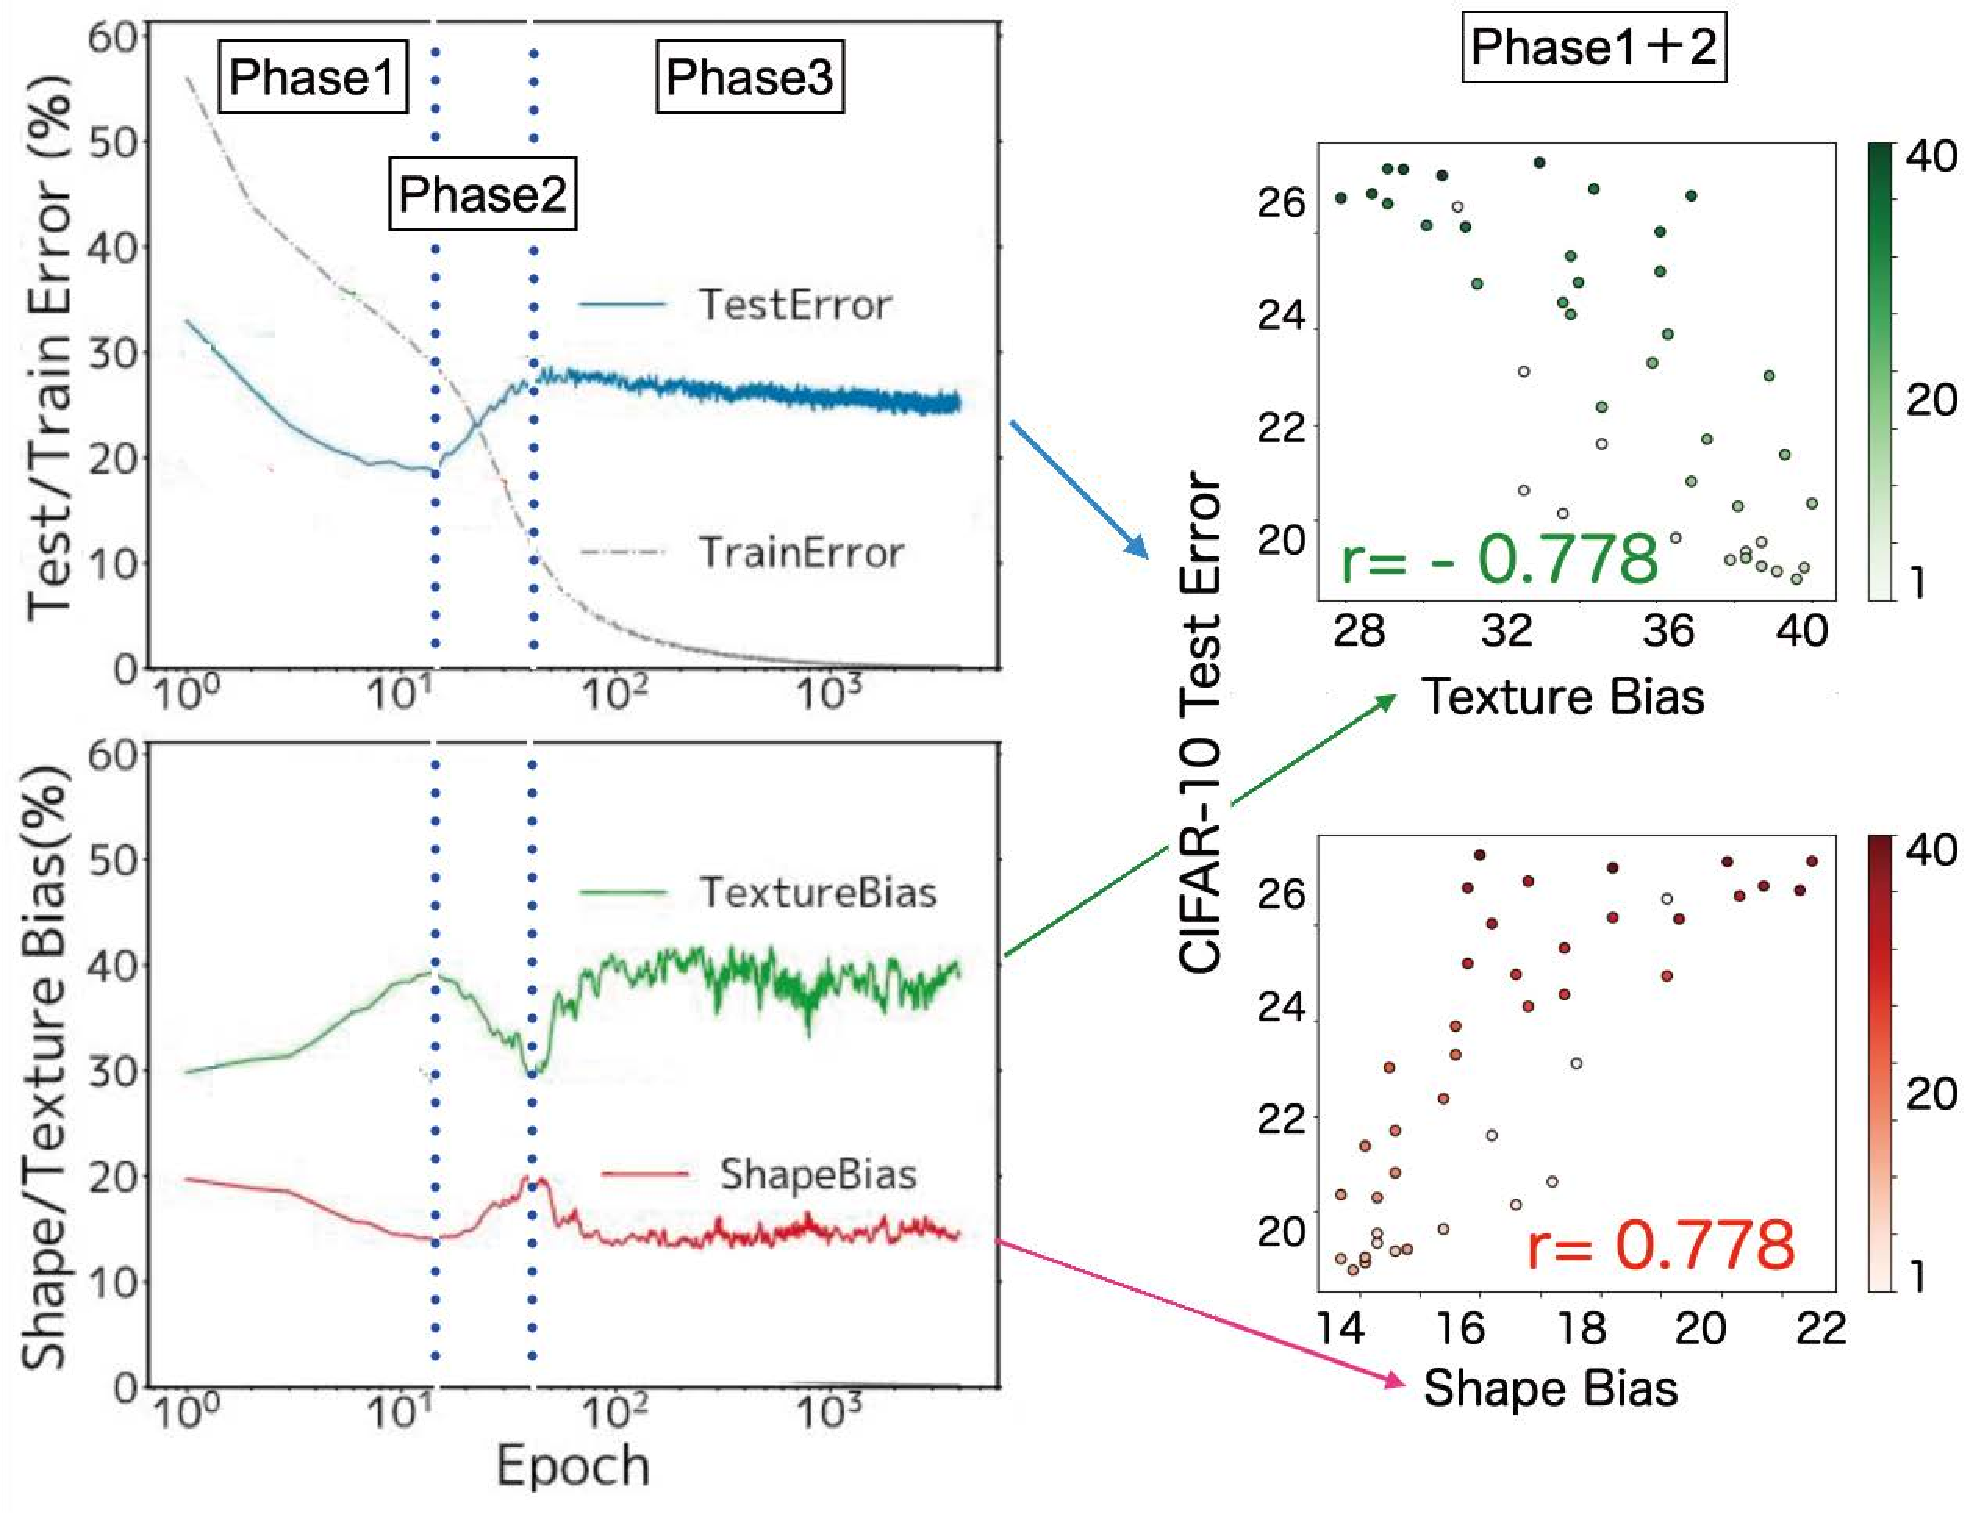
\includegraphics[width=1.0\columnwidth]{fig/result_overview.pdf}
\caption[Schematic overview of this study.]{
% 図2.本研究の概要を示す模式図.左上: 二重降下(DD)が観測されたCIFAR-10画像認識タスクの学習曲線;テスト誤差はその時間的分化に基づいて3つのPhaseに分けられた.実験結果はnakiranらによる既報[18]と同条件でDDを再現した結果である.左下: 前述の学習過程におけるモデルの形状/テクスチャの偏りを記録したもの.テスト誤差と形状・テクスチャの偏りの同期的変化を示す.右: テストエラーと形状/テクスチャバイアスの散布図.特にPhase 1とPhase 2において,テストエラーと形状バイアスの間には正の相関があり,テストエラーとテクスチャバイアスの間には負の相関がある.
Schematic overview of this study. Top left: Learning curve of the CIFAR-10 image recognition task where double descent was observed; test errors were divided into three phases based on their temporal differentiation. The experimental results are a reproduction of double descent under the same conditions as previously reported by Nakiran \textit{et al.}\cite{nakkiran2021deep}. Bottom left: This records the model's shape/texture bias during the aforementioned learning process. It shows the synchronous changes between test errors and shape/texture biases. Right: A scatter plot of test error and shape/texture bias. Especially in Phase 1 and Phase 2, there is a positive correlation between test error and shape bias, and a negative correlation between test error and texture bias.
% Schematic illustration showing the outline of this study.Top left: Learning curve depicting the CIFAR-10 image recognition task with observed double descent (DD); the test error was divided into three phases based on its temporal differentiation.The experimental results are the results of reproducing DD under the same conditions as in the previous report by nakiran \textit{et al.}\cite{nakkiran2021deep}.Bottom left: Recorded shape/texture biases of the model during the aforementioned learning process.Observations indicate synchronous changes in test error and shape/texture biases.Right: Scatter plot representing test error and shape/texture bias values for the interval encompassing phases 1 and 2, revealing a positive correlation between test error and shape bias, as well as a negative correlation between test error and texture bias.
}
\label{fig:overview}
\end{figure}

\newpage

\section[Correlation analysis in each phase of the double descent]{
Correlation analysis in each phase of the double descent (\cref{tab:base_condition_result})
}
4.3節で定義したPhase1,Phase2,Phase3におけるテスト誤り率と形状・テクスチャ偏重度の相関係数を計算し,より詳細な評価を行った.これらの結果を\cref{tab:base_condition_result}に示す.Phase1とPhase2におけるテスト誤り率と形状偏重度との相関係数はそれぞれ0.898と0.771であり,正の相関があることがわかる.逆に,Phase1とPhase2におけるテスト誤り率とテクスチャ偏重度との相関係数は\textminus0.829と\textminus0.797であり,負の相関を示している.Phase3では,形状偏重度の相関値は\textminus0.026,テクスチャ偏重度の相関値は0.118であり,相関は見られなかった.これらの結果から,Phase1と2では相関が見られたが,Phase3では相関が見られなかった.形状とテクスチャの関係を簡単に理解するために,形状とテクスチャの相関値をScoreと呼ばれる指標で表す.Scoreは,これらの相関係数の絶対値の平均である.Scoreが高いほど,テスト誤り率と形状/テクスチャ偏重度それぞれとの相関が強いことを示す.以降の実験では,今回の条件において高い相関を示したPhase1,2とPhase3それぞれの区間で相関係数とScoreを算出し,定性的な分析に利用する.

\begin{table}[h]
\centering
    \caption[The correlation coefficients and scores for the three phases]{
    % 定義した方法(\cref{sec:Phase division of double descent})によって分けた3つのPhaseの相関係数とスコア.相関係数を計算するために使用された実際のデータ間隔(Epoch range),Test ErrorとShape biasから計算された相関係数,Test ErrorとTexture biasから計算された相関係数,2つの相関係数から計算された相関スコアを示している.
    The correlation coefficients and scores for the three phases divided according to the method defined in (\cref{sec:Phase division of double descent}). It shows the Epoch range used to calculate the correlation coefficients, the correlation coefficients calculated from Test Error and Shape bias, the correlation coefficients calculated from Test Error and Texture bias, and the correlation score computed from these two correlation coefficients.
    % Correlation coefficients and scores for the three phases, divided by \cref{sec:Phase division of double descent}. The following table shows the actual data interval used to compute the correlation coefficients (Epoch range), the correlation coefficient computed from the Test Error and the Shape corr, the correlation coefficient computed from the Test Error and the Texture corr, and the correlation score computed from the two correlation coefficients.score calculated from the two correlation coefficients.
    }
    
    \scalebox{1.2}{
    \begin{tabular}{c|c|SS|c}
    \toprule[0.8pt]
     Phase & Epoch range & {Shape corr}& {Texture corr}& Score\\
     \midrule[0.5pt]
    Phase1 & 2 - 12 &0.898 &-0.829 &0.863\\
    Phase2 & 12 - 41&0.771& -0.797&0.784\\
    Phase3 & 41 - 1,000&-0.026 & 0.118&0.072\\
    \toprule[0.8pt]
    \end{tabular}
    }
    \label{tab:base_condition_result}
    % \vspace{-15pt}
\end{table}

\newpage

\section{詳細なアブレーション実験}
\subsection{概要}
本節では,先に述べた条件から一部を変更し,実験を構成する各条件が二重降下と偏重度の推移にどのように影響を与えるかを検証する.具体的には,以下の条件を変更した: "事前学習の有無","使用データセット","ResNet Family内でのモデル変更","使用CNNモデル","バッチサイズ","ラベルノイズの割合","シード値".実際に変更した条件と該当する図の一覧を\cref{tab:ablation_list}に示す.以降の実験では,実験の高速化のために,学習回数を1,000 epochとした.

\begin{table}[h]
\centering
    \caption[List of changed conditions and corresponding fig. numbers in ablation studys.]{List of changed conditions and corresponding fig. numbers in ablation studys.This table shows only the conditions changed from the base in bold.Blank spaces indicate the same as above.}
    \scalebox{1.1}{
    \begin{tabular}{c|c|c|c|c|c|c}
    \toprule[0.8pt]
    pre-train & Model & dataset & batchsize & Label Noise & seed & Fig. No\\
     \midrule[0.5pt]
    ImageNet & ResNet18 & CIFAT-10 & 128 & 0.2 & 42 & \ref{fig:overview}\\
    \midrule[0.1pt]
    \textbf{None}& ResNet18 & CIFAT-10 & 128 & 0,2 & 42 & \ref{fig:comp_INSR}\\
    ImageNet &          & \textbf{CIFAT-100}&     &     &    & \ref{fig:comp_IN_dataset}\\
             &\textbf{ResNet34} & CIFAT-10 &     &     &    & \ref{fig:comp_model}\\
             &\textbf{ResNet50} &          &     &     &    & \ref{fig:comp_model}\\
             &\textbf{DenceNet} &          &     &     &    & \ref{fig:comp_cnn_model}\\
             &\textbf{MobileNet}&          &     &     &    & \ref{fig:comp_cnn_model}\\
             &\textbf{EfficientNet}&       &     &     &    & \ref{fig:comp_cnn_model}\\
             & ResNet18 &          &  \textbf{8} &     &    & \ref{fig:comp_batchsize}\\
             &          &          &  \textbf{16} &     &    & \ref{fig:comp_batchsize}\\
             &          &          &  \textbf{64} &     &    & \ref{fig:comp_batchsize}\\
             &          &          & 128 & \textbf{0.4} &    & \ref{fig:comp_ln}\\
             &          &          &     & \textbf{0.6} &    & \ref{fig:comp_ln}\\
             &          &          &     & 0.2 &  \textbf{0} & \ref{fig:comp_seed}\\
             &          &          &     &     &  \textbf{1} & \ref{fig:comp_seed}\\
    \toprule[0.8pt]
    \end{tabular}
    }
    \label{tab:ablation_list}
\end{table}

\newpage

\subsection[Init parameter]{Init parameter (see \cref{fig:comp_INSR})}
ベースラインの条件では,先行研究において,ImageNetにおける学習の文脈で形状・テクスチャに関する研究が行われていたことを考慮し,ImageNet-1kの学習済みパラメータをモデルの初期値として用いた.本実験では,ImageNet-1kとランダム値(Scratch)を比較することで,初期値に基づく形状とテクスチャの偏りの関係を検証した.その結果を\cref{fig:comp_INSR}に示す.この結果から,ImageNet-1kの初期パラメータを用いた場合,形状・テクスチャ偏重度が明瞭に変化することがわかる.このような結果になった理由の1つとして,ImageNetを事前学習することで得られる特徴表現と,CIFAR-10を学習することで得られる特徴表現が大きく異なることが考えられる.それによって,ImageNetを事前学習したパラメータの状態から,CIFAR-10に適応するために,大きくパラメータの状態が変化し,その結果偏重度の推移の変化として現れたと考えられる.また,Scratchを用いた場合においても,二重降下のPhase 1からPhase 2への移り変わりにおいて,特にテクスチャ偏重度はわずかながら上昇から下降に転じているように見受けられる.そのため,双方の条件において,学習傾向の移り変わりが起きている可能性が考えられる.しかし,CIFAR-10の学習時に,ImageNetで事前学習した場合に,二重降下と同期したような挙動を強くすることは,非常に興味深い現象である.このような差異について,パラメータが如何に変化していっているかという点が重要であると考えられる.
% ベースラインの条件では,先行研究において,ImageNetにおける学習の文脈で形状・テクスチャに関する研究が行われていたことを考慮し,ImageNet-1kの学習済みパラメータをモデルの初期値として用いた.本実験では,ImageNet-1kとランダム値(Scratch)を比較することで,初期値に基づく形状とテクスチャの偏りの関係を検証した.その結果を\cref{fig:comp_INSR}に示す.この結果から,ImageNet-1kの初期パラメータを用いた場合,形状・テクスチャ偏重度が明瞭に変化することがわかる.しかし,Scratchを用いると,特徴的な変化は生じない.このような結果になった理由の1つとして,ImageNetを事前学習することで得られる特徴表現と,CIFAR-10を学習することで得られる特徴表現が大きく異なることが考えられる.それによって,ImageNetを事前学習したパラメータの状態から,CIFAR-10に適応するために,大きくパラメータの状態が変化し,その結果偏重度の推移の変化として現れたと考えられる.しかし,CIFAR-10の学習時に,ImageNetで事前学習した場合だけ,偏重度が一定で推移せず,二重降下と同期したような挙動をすることは,非常に興味深い現象である.
% 本実験では,ImageNetで事前学習した場合とランダム値(Scratch)を比較することで,初期値に基づく形状とテクスチャの偏りの関係を調べた.その結果を\cref{fig:comp_INSR}に示す.この結果から,ImageNetで事前学習した場合に限って,形状・テクスチャ偏重度が特異に変化することがわかる.しかし,Scratchを用いると,特徴的な変化は生じない.このような結果になった理由の1つとして,事前学習で得た特徴から新たなデータに適合するににあたって,偏重度の特異な推移という形で現れていると考えられる.

\begin{figure}[htb]
\centering
   \begin{tabular}{cc}
      %---- 最初の図 ---------------------------
      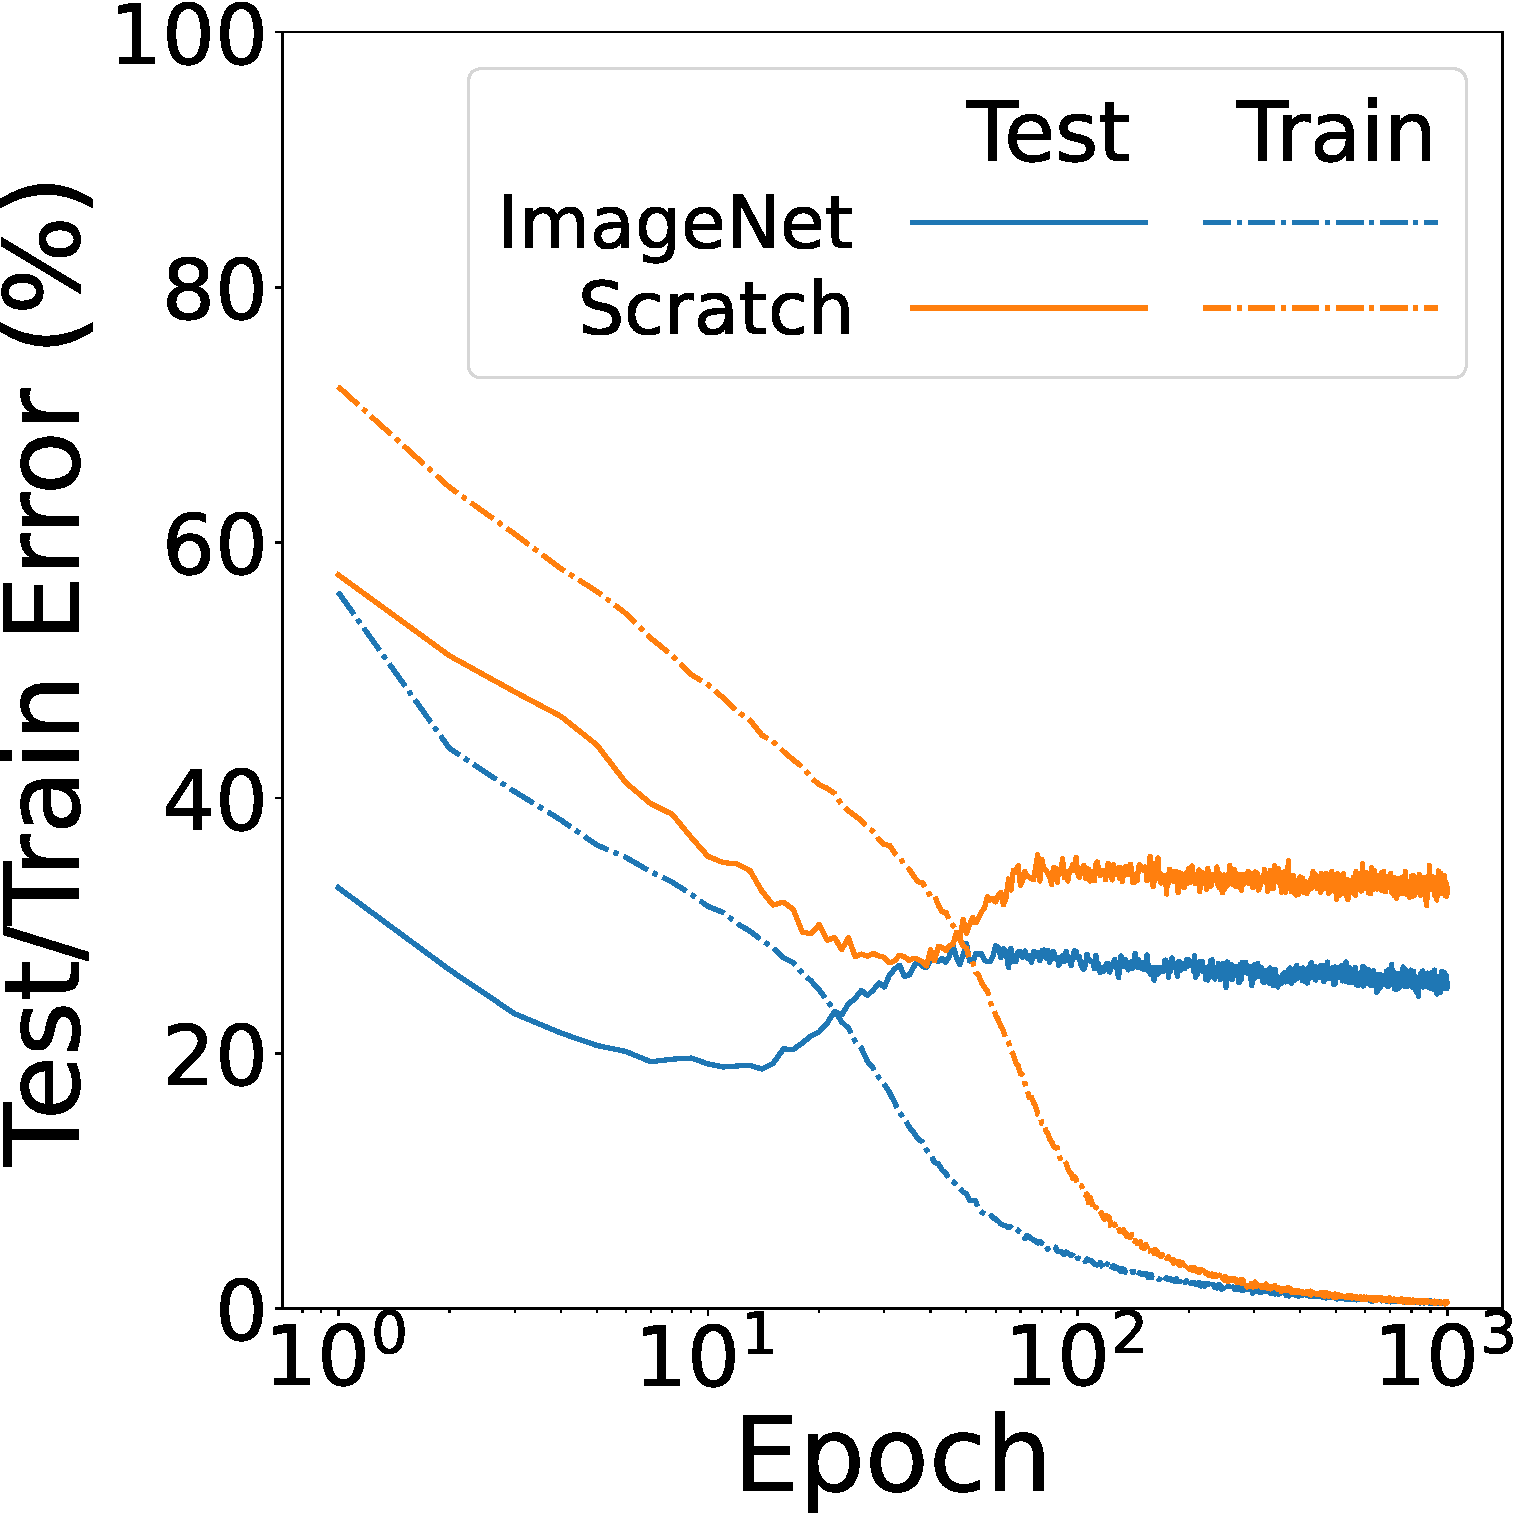
\includegraphics[keepaspectratio, width=0.45\linewidth]{fig/INSR_learning_curv.pdf} &
      \hspace{5pt}
      %---- 2番目の図 --------------------------
      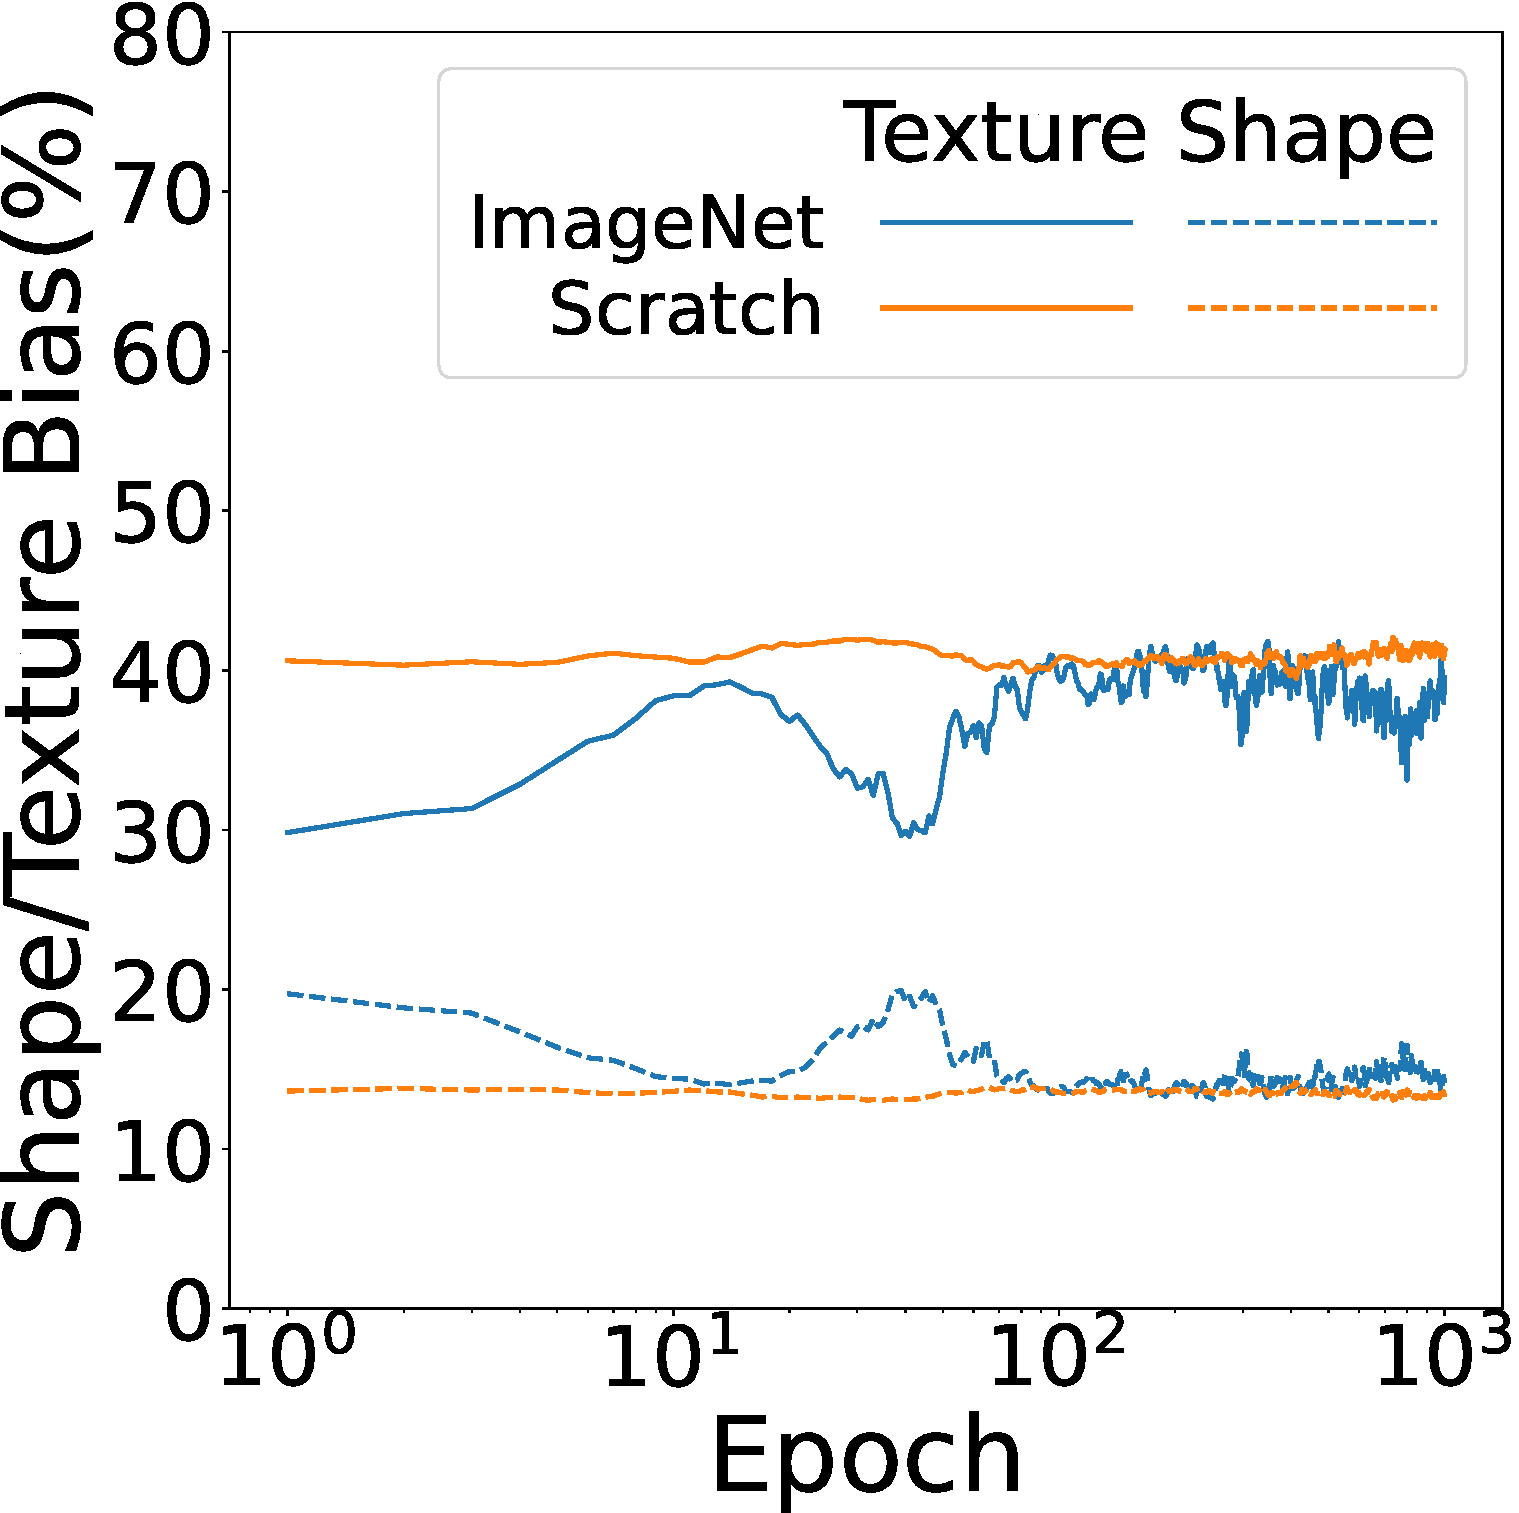
\includegraphics[keepaspectratio, width=0.45\linewidth]{fig/INSR_sha_tex.pdf}
   \end{tabular}
\caption[Learning process with and without pretraining by ImageNet.]{Learning process with and without pretraining by ImageNet. Left: train/test errors Right: shape/texture bias values.}
%Learning curve graphs for double descent and shape/texture bias with and without pretraining on ImageNet. \textbf{Left}:learning curve. \textbf{Right}:model's bias shift.}
\label{fig:comp_INSR}
\end{figure}

\newpage

\subsection[Dataset]{Dataset (\cref{fig:comp_IN_dataset} and \cref{tab:corr_FTdataset})}
データセットを変更した場合の影響を調査するために,CIFAR-10と性質が類似しているCIFAR-100で学習し,CIFAR-10の場合と差異を検証した.結果を\cref{fig:comp_IN_dataset}に,定量評価を\cref{tab:corr_FTdataset}に示す.その結果,CIFAR-10では,Phase1とPhase2において,形状の偏りとの相関は0.778であり,テクスチャの偏りとの相関は-0.778であった.一方,CIFAR-100では,形状の偏りとの相関は-0.689,テクスチャの偏りとの相関は0.745となり,逆相関の関係を示した.CIFAR-10,100ともに,Phase3における形状とテクスチャの相関は,スコア結果からほぼ無視できる.CIFAR-100で観測された逆の相関は,クラス数,クラスの種類,1クラスあたりの枚数などの要因に影響されたCIFAR-10,CIFAR-100特有の特性の差異によるものであると推測される.一方で,逆相関をみせることから,二重降下と偏重度の推移に相関を引き起こす,共通の特性が存在する可能性を示唆している.

また,CIFAR-100から10クラスを抜き出して同様の実験を行った場合にも,CIFAR-100の場合と類似した形状・テクスチャ偏重度の推移を示した.これによってクラス数の差異が直接関係しているわけではないと考えられる.CIFAR-100は20の上位クラスとそれぞれに含まれる5つの下位クラスで構成されている.そのため,たとえば,魚の上位クラスあり,その上位クラスには魚の質感をした5つのクラスが含まれていることになる.それによってCIFAR-10とは重視される特徴に差異が出ている可能性が考えられる.
% データセットを変更した場合の影響を調査するために,CIFAR-10と性質が類似しているCIFAR-100で学習し,CIFAR-10の場合と差異を検証した.結果を\cref{fig:comp_IN_dataset}に,定量評価を\cref{tab:corr_FTdataset}に示す.その結果,CIFAR-10では,Phase1とPhase2において,形状の偏りとの相関は0.778であり,テクスチャの偏りとの相関は-0.778であった.一方,CIFAR-100では,形状の偏りとの相関は-0.689,テクスチャの偏りとの相関は0.745となり,逆相関の関係を示した.CIFAR-10,100ともに,Phase3における形状とテクスチャの相関は,スコア結果からほぼ無視できる.CIFAR-100で観測された逆の相関は,クラス数,クラスの種類,1クラスあたりの枚数などの要因に影響されたCIFAR-10,CIFAR-100特有の特性の差異によるものであると推測される.一方で,逆相関をみせることから,二重降下と偏重度の推移に相関を引き起こす,共通の特性が存在する可能性を示唆している.

\begin{figure}[htb]
\centering
%    \begin{tabular}{c}
%     %---- 最初の図 ---------------------------
%      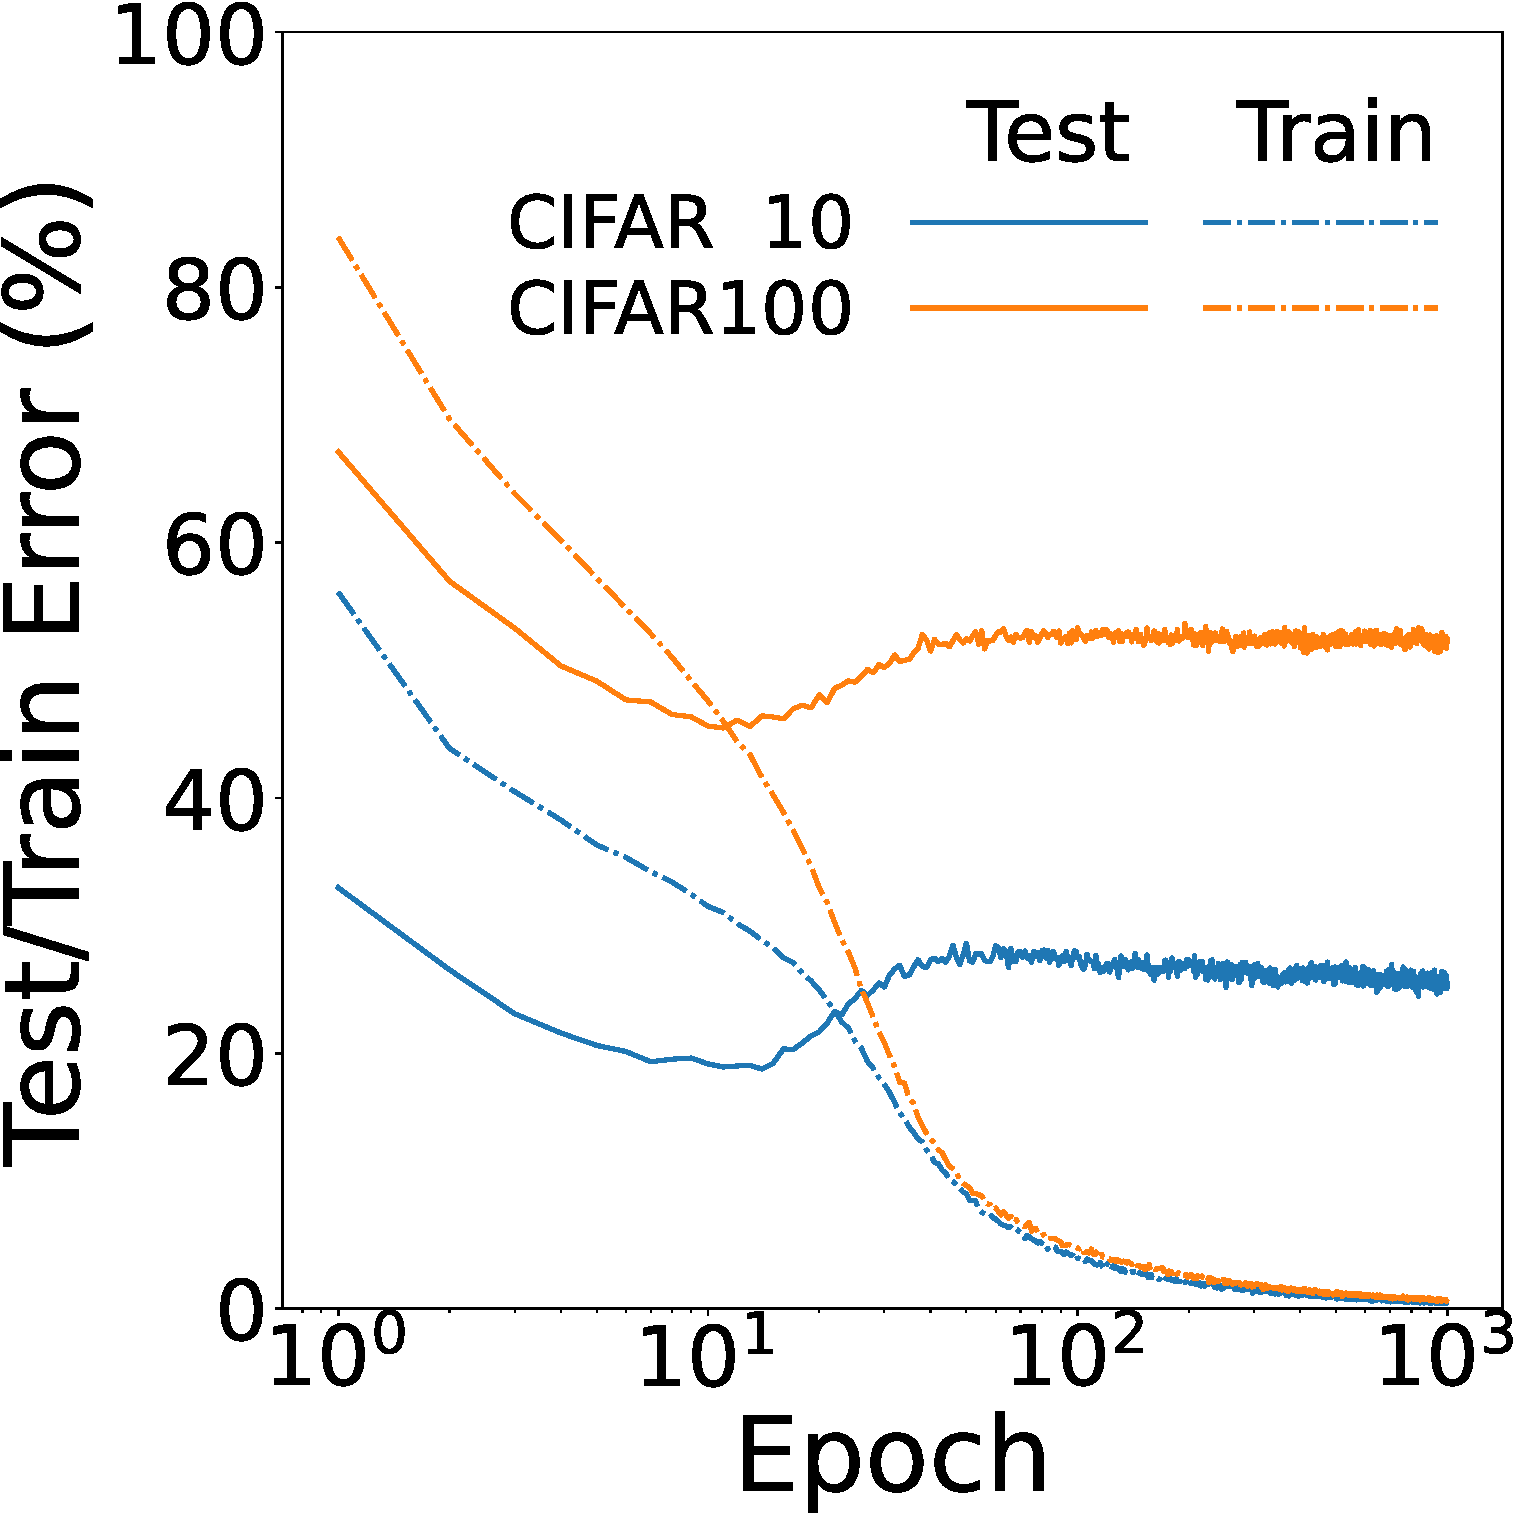
\includegraphics[keepaspectratio, width=0.458\linewidth]{fig/IN_dataset_learning_curv.pdf}
%      %---- 2番目の図 --------------------------
%      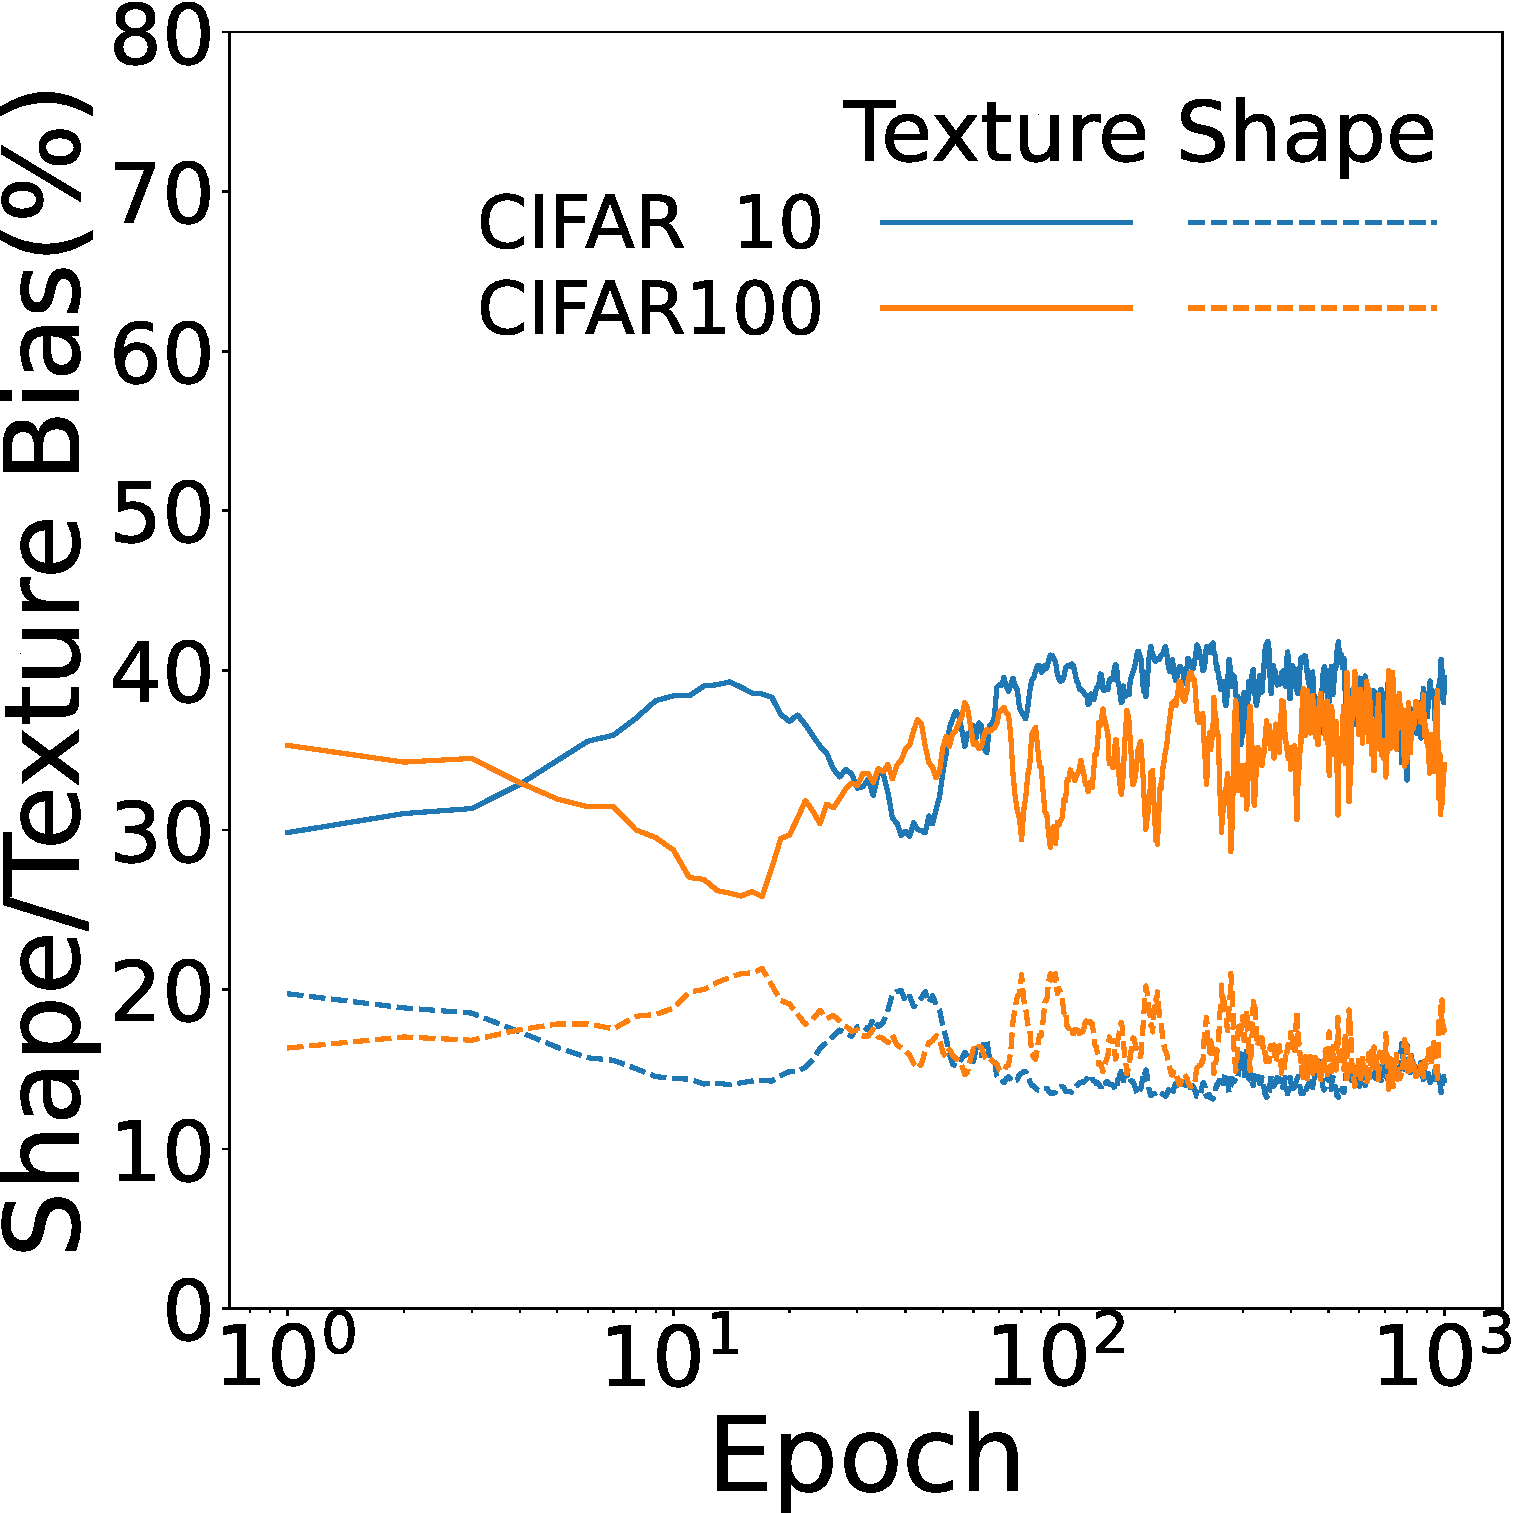
\includegraphics[keepaspectratio, width=0.458\linewidth]{fig/IN_dataset_sha_tex.pdf}
%    \end{tabular}
    \begin{tabular}{cc}
      %---- 最初の図 ---------------------------
      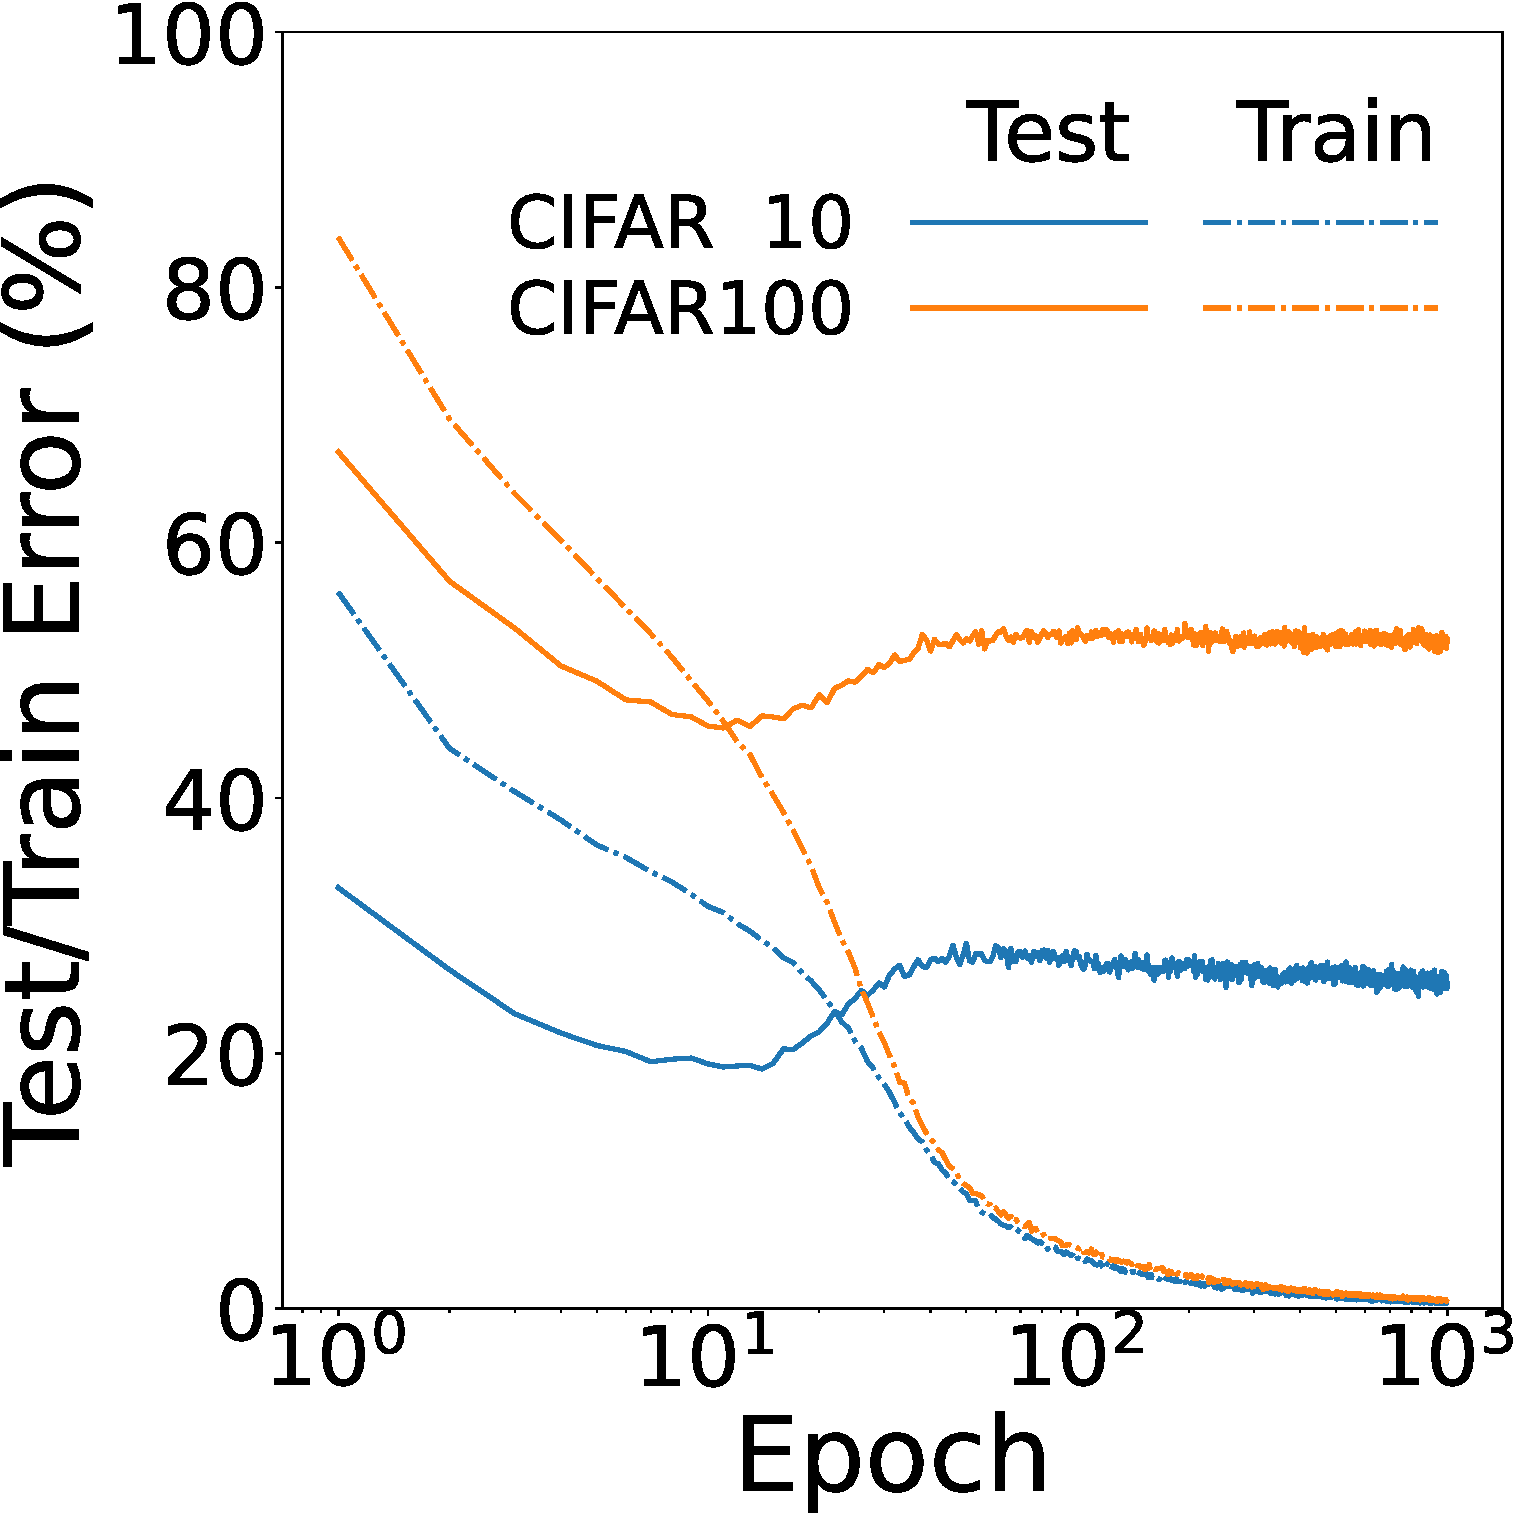
\includegraphics[keepaspectratio, width=0.45\linewidth]{fig/IN_dataset_learning_curv.pdf} &
      \hspace{5pt}
      %---- 2番目の図 --------------------------
      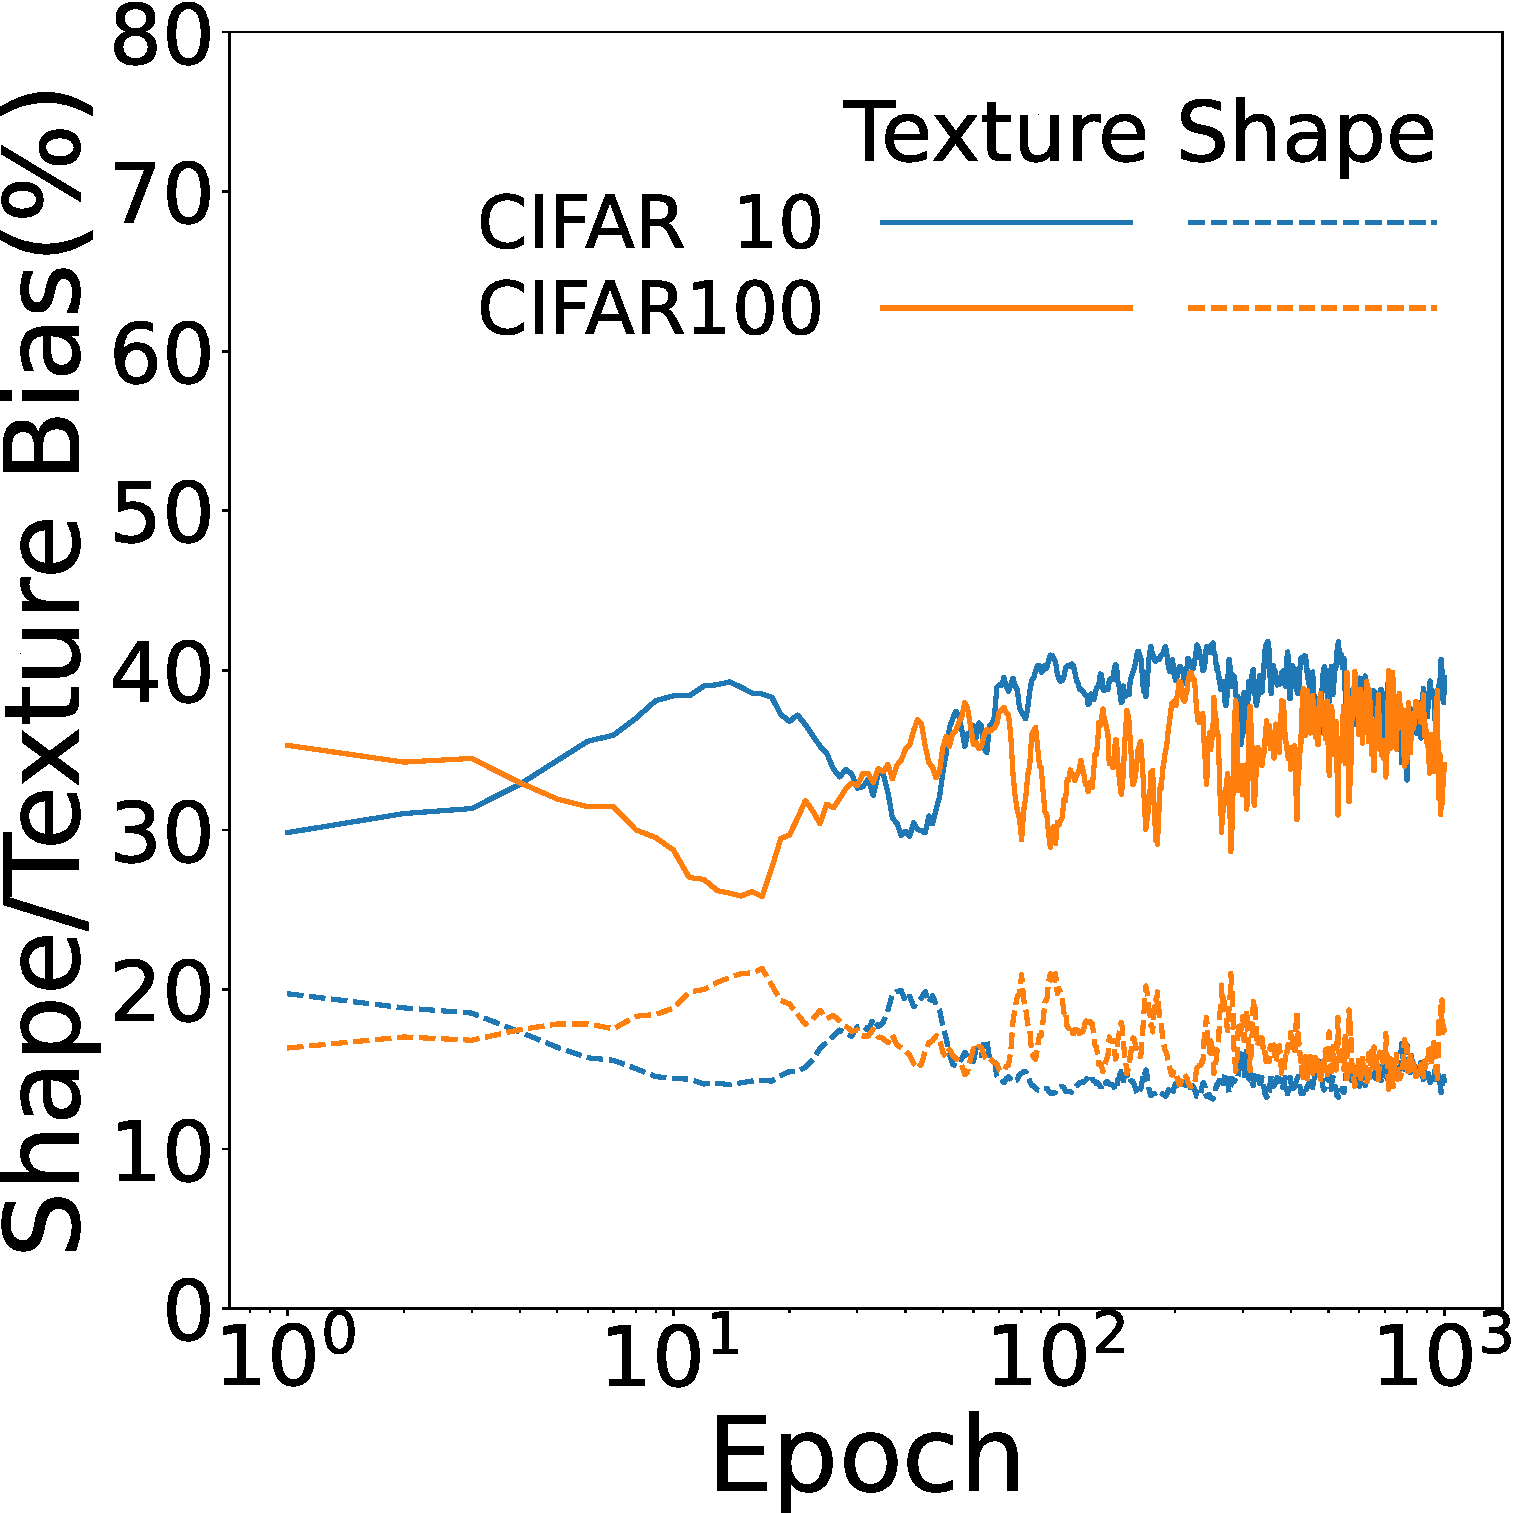
\includegraphics[keepaspectratio, width=0.45\linewidth]{fig/IN_dataset_sha_tex.pdf}
    \end{tabular}
\caption[Learning process by different tasks, CIFAR-10 and CIFAR-100.]{Learning process by different tasks, CIFAR-10 and CIFAR-100. Left: train/test errors Right: shape/texture bias values.
%Learning curve graphs for double descent and shape/texture bias for different datasets. \textbf{Left}:learning curve. \textbf{Right}:model's bias shift.
% Epoch-wise double descent vs model's shape/texture bias shift in fine-tuning dataset differences. \textbf{Left}:learning curve. \textbf{Right}:model's bias shift.
}
\label{fig:comp_IN_dataset}
\end{figure}

\begin{table}[htb]
    \centering
    \caption{
    % sample
    % 各ステージ毎の相関係数.相関係数を計算するために利用したデータの区間およびTest Errorと形状偏重度で計算した相関係数(Shape corr),TestErrorとテクスチャ偏重度で計算した相関係数(Texture corr)及び二つの相関係数から計算した最終的なスコアを示している.
    % 各データセットでfine-tuningした場合におけるPhase1, 2,およびPhase3での相関係数とscore.Test errorとShape biasとの相関係数(SB),Test errorとTexture biasとの相関係数(TB)及び二つの相関係数から計算したscoreを示している.
    Correlation coefficients and scores in Phase 1, 2 and Phase 3 for different datasets.
    }
    %old version
    % \begin{tabular}{c|c|c} 
    % \toprule[0.8pt]
    % Datasets  &  Correlation area &  score\\
    %  \midrule[0.5pt]
    % CIFAR10  & Stage1,2 (2-41) &0.778\\
    % CIFAR100 & Stage1,2 (2-55) &0.717\\
    % \toprule[0.8pt]
    % \end{tabular}
    % \label{tab:corr_FTdataset}
    \scalebox{1.2}{
    \begin{tabular}{c|SSc|SSc} 
    \toprule[0.8pt]
    \multirow{2}{*}{CNN}  &  \multicolumn{3}{c|}{Correlation of Phase1,2} &  \multicolumn{3}{c}{Correlation of Phase3}\\
     \cline{2-7}
             & {SB} & {TB} & Score & {SB} & {TB} & Score \\
     \midrule[0.5pt]
    C10  &0.778&-0.778 & 0.778 & -0.026&0.118 & 0.072\\
    C100 &-0.689&0.745 & 0.717&0.002&0.013 & 0.007\\
    \toprule[0.8pt]
    \end{tabular}
    }
    \label{tab:corr_FTdataset}
\end{table}

\newpage

\subsection[ResNet family]{ResNet family (see \cref{fig:comp_model} and \cref{tab:corr_model})}
モデルのパラメータ数の影響,特にResNet family内で一般性があるのかを検証するため,ResNet18と同様の論文で提案されているResNet34,ResNet50でも実験を行った.使用するモデルをResNet34,ResNet50に変更した場合の結果を\cref{fig:comp_model}に,定量的な評価のための表を\cref{tab:corr_model}に示す.ResNet34においては,偏重度の推移に相関があるように見られ,Phase1,2のScoreが0.517とResNet18の場合と同様の相関を定量的にも示す.しかし,ResNet50においては,偏重度の推移には定性的にはPhase2での変化が見られず,定量的にも相関がみられない.この結果の理由として,ResNetは,ResNet18,ResNet34,ResNet50とパラメータ数が増加するため,パラメータ数の上昇に従って,相関が消える可能性が考えられる.また,使用したResNetの構造の差異を考えると,ResNet18,ResNet34はbasic blockと呼ばれる構造から形成されているのに対して,ResNet50はbottleneckと呼ばれる構造から形成されており,この点が影響を与えた可能性も考えられる.

\begin{figure}[htb]
\centering
   \begin{tabular}{cc}
      %---- 最初の図 ---------------------------
      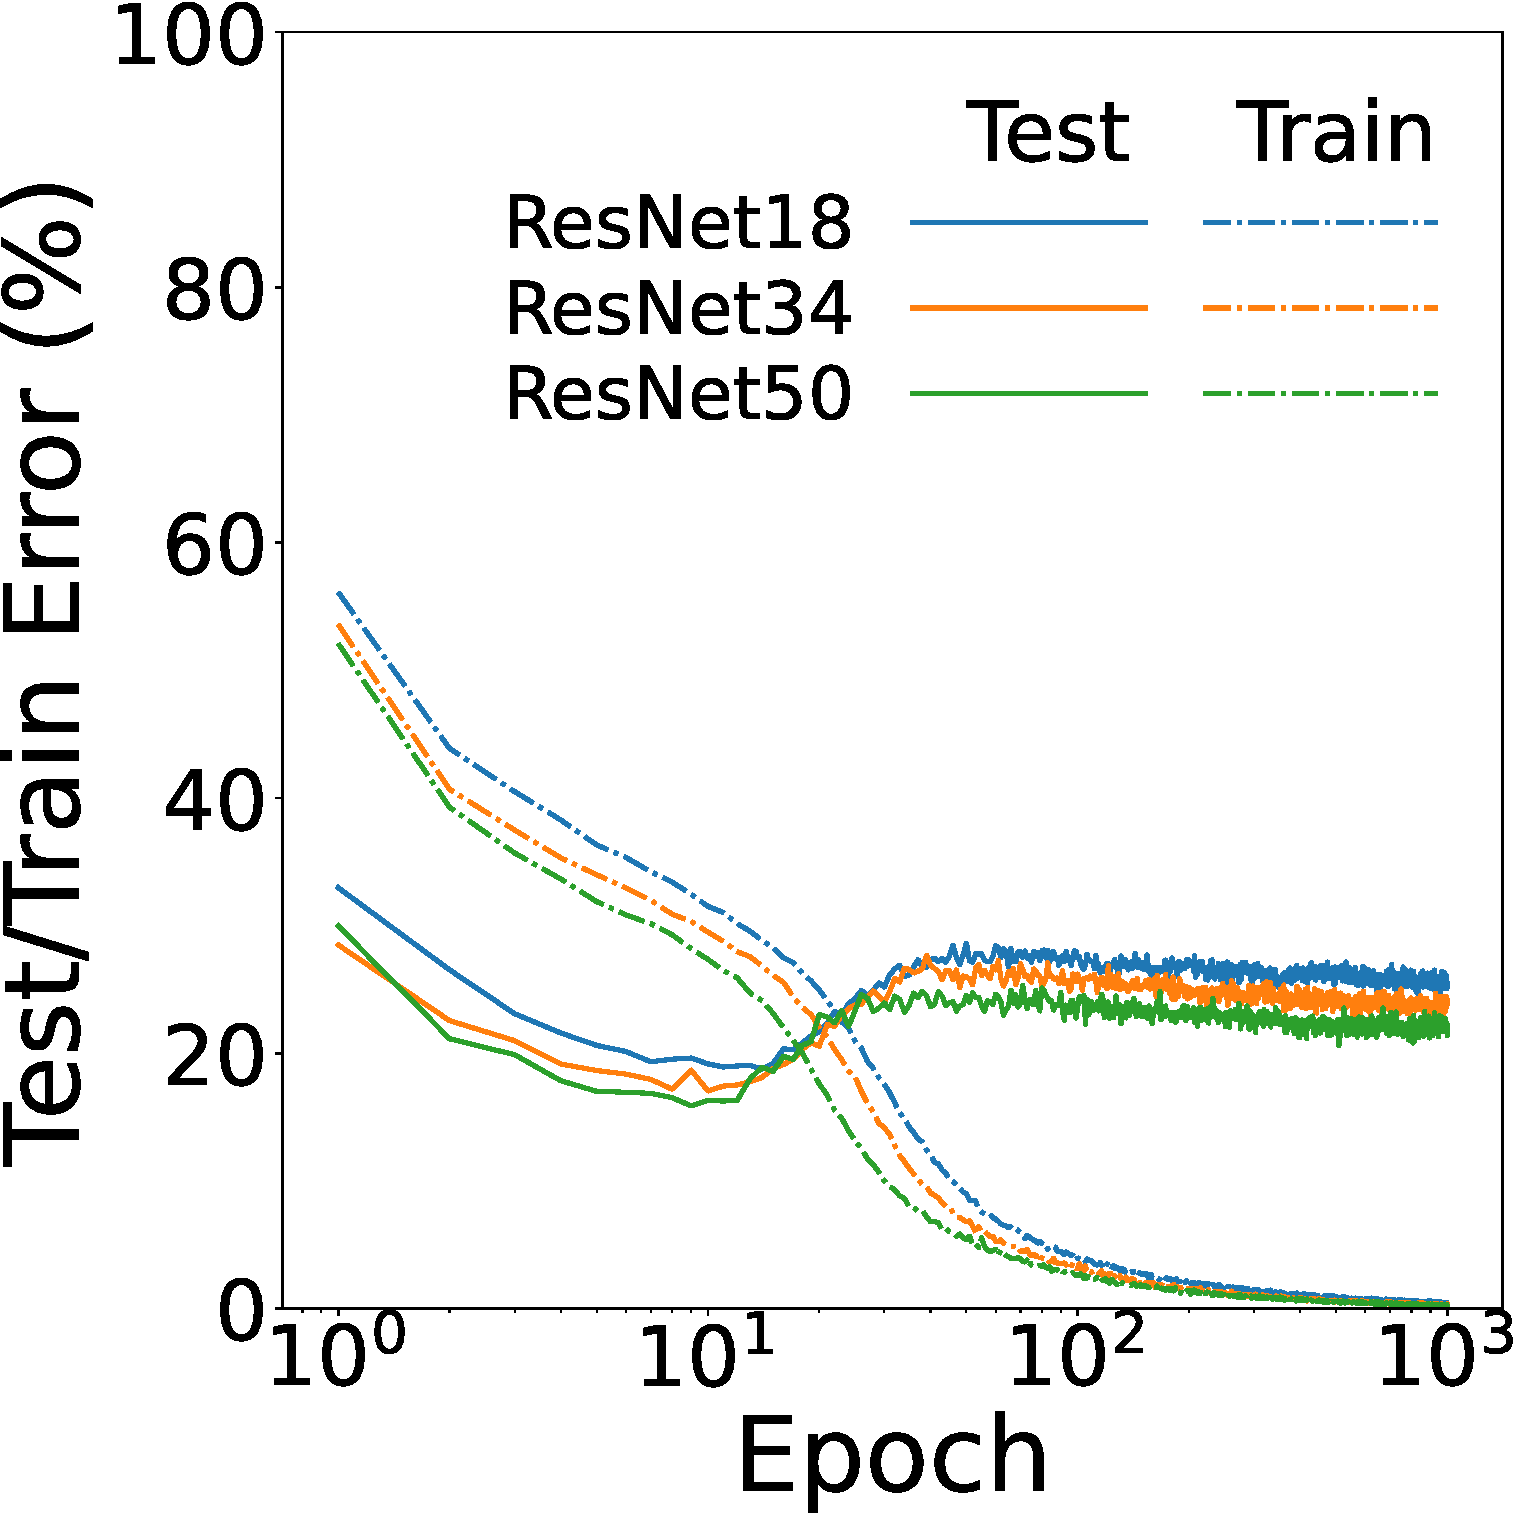
\includegraphics[keepaspectratio, width=0.45\linewidth]{fig/model_learning_curv.pdf} &
       \hspace{5pt} 
      %---- 2番目の図 --------------------------
      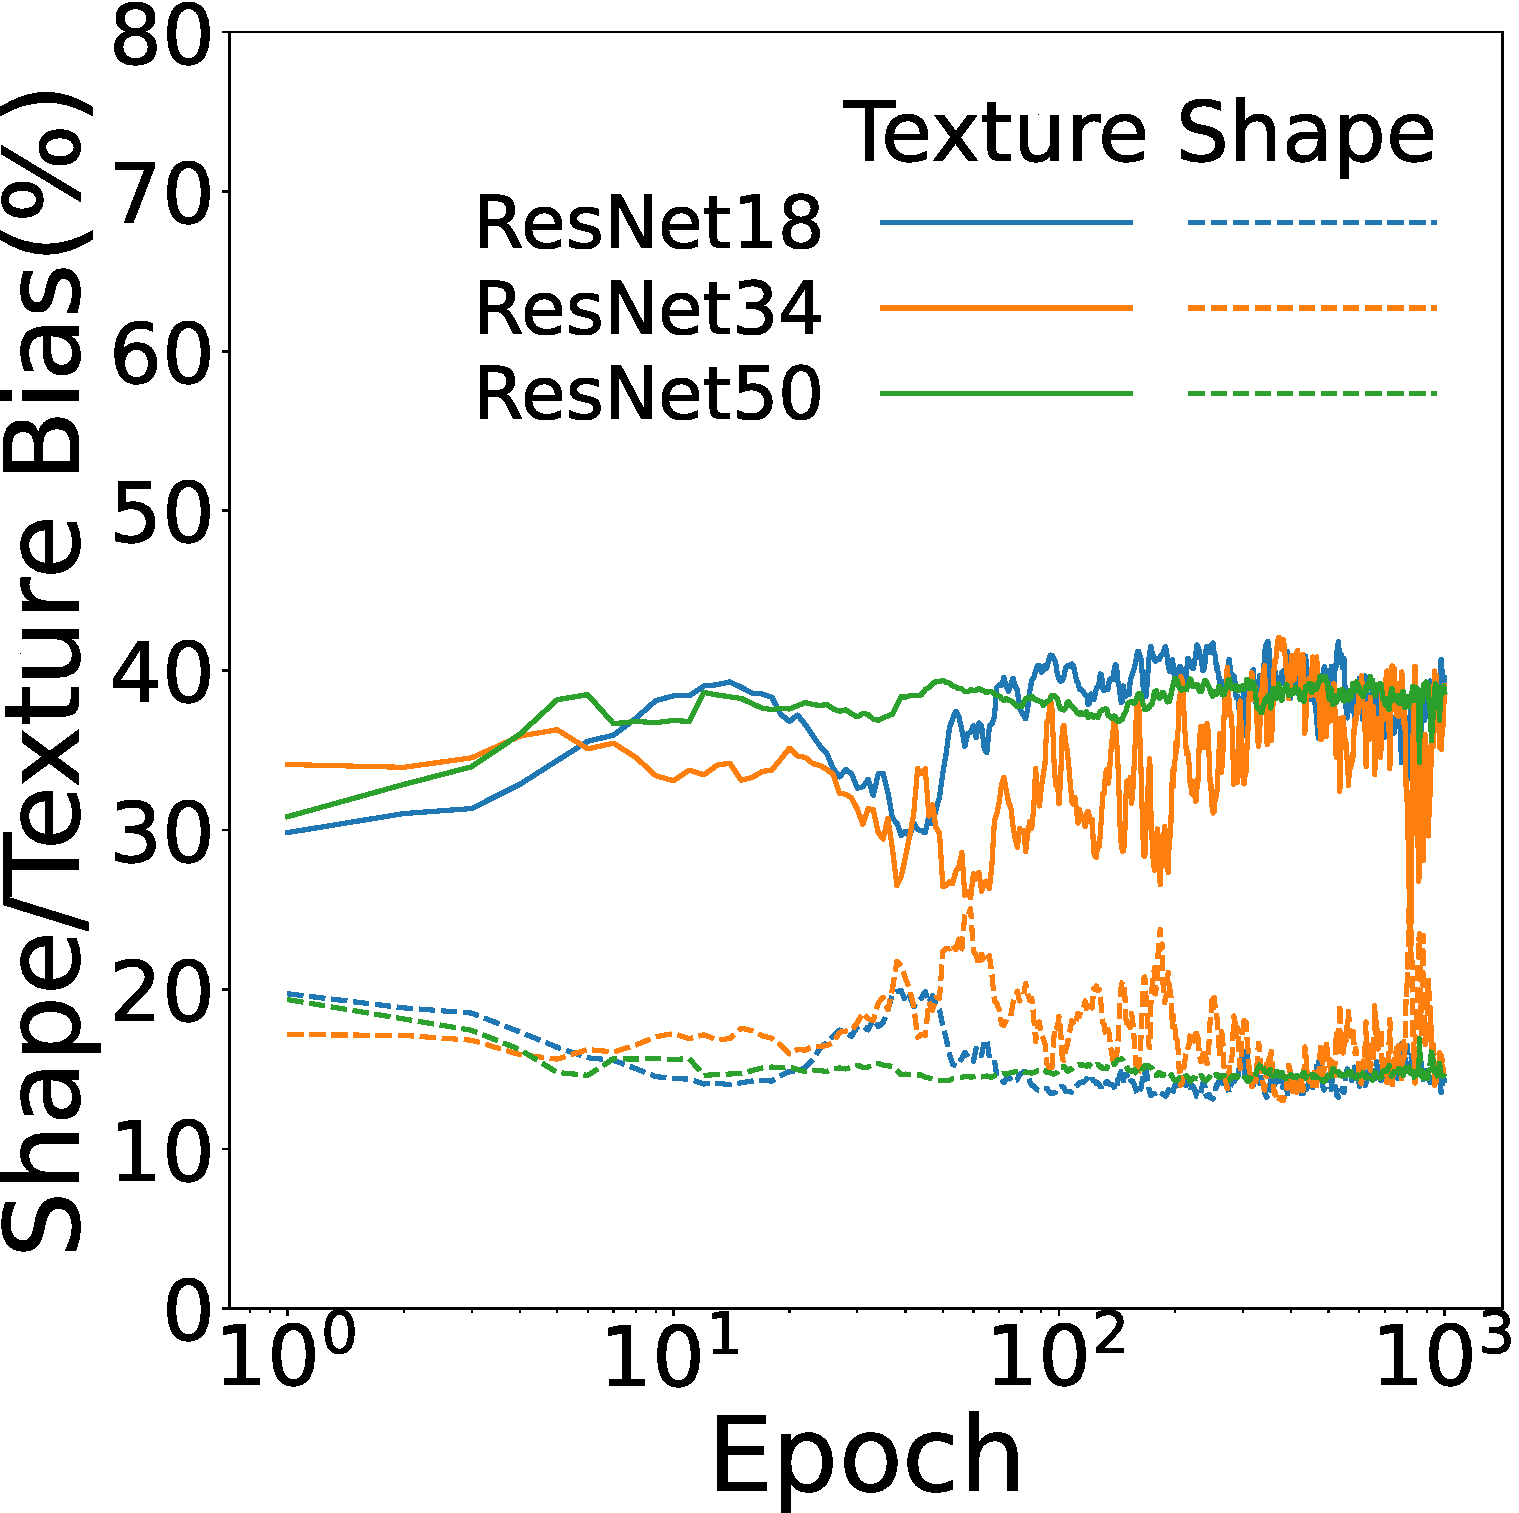
\includegraphics[keepaspectratio, width=0.45\linewidth]{fig/model_sha_tex.pdf}
   \end{tabular}
\caption[Learning process under various size conditions of ResNet family.]{
Learning process under various size conditions of ResNet family. Left: train/test errors Right: shape/texture bias values.}
% Learning curve graphs for double descent and shape/texture bias for different models. \textbf{Left}:learning curve. \textbf{Right}:model's bias shift.}
\label{fig:comp_model}
\end{figure}

\begin{table}[htb]
    \centering
    \caption{
    % sample
    % 各ステージ毎の相関係数.相関係数を計算するために利用したデータの区間およびTest Errorと形状偏重度で計算した相関係数(Shape corr),TestErrorとテクスチャ偏重度で計算した相関係数(Texture corr)及び二つの相関係数から計算した最終的なスコアを示している.
    % 各モデルを使用した場合におけるPhase1, 2,およびPhase3での相関係数とscore.Test errorとShape biasとの相関係数(SB),Test errorとTexture biasとの相関係数(TB)及び二つの相関係数から計算したscoreを示している.
    Correlation coefficients and scores in Phase 1, 2 and Phase 3 for different ResNet Family.
    }
    % \begin{tabular}{c|c|c} 
    % \toprule[0.8pt]
    % Model  & Correlation area&  score\\
    %  \midrule[0.5pt]
    % ResNet18  & Stage1,2 (2-41) &0.778\\
    % ResNet34 & Stage1,2 (2-41) &0.517\\
    % ResNet50 & Stage1,2 (2-180) &0.215\\
    % \toprule[0.8pt]
    % \end{tabular}
    \scalebox{1.2}{
    \begin{tabular}{c|SSc|SSc} 
    \toprule[0.8pt]
    \multirow{2}{*}{CNN}  &  \multicolumn{3}{c|}{Correlation of Phase1,2} &  \multicolumn{3}{c}{Correlation of Phase3}\\
     \cline{2-7}
             & {SB} & {TB} & Score & {SB} & {TB} & Score \\
     \midrule[0.5pt]
    ResNet18 &0.778&-0.778 & 0.778 & -0.026&0.118 & 0.072\\
    ResNet34 &0.498& -0.536 & 0.517 & 0.165 & -0.281 & 0.223\\
    ResNet50 &-0.153&0.136& 0.144 & -0.097&0.064 & 0.080\\
    \toprule[0.8pt]
    \end{tabular}
    }
    \label{tab:corr_model}
\end{table}

\newpage

\subsection[CNN models]{CNN models (see \cref{fig:comp_cnn_model} and \cref{tab:corr_CNN_model})}
ResNetとは異なるCNNモデルを使用した場合における,二重降下と形状・テクスチャ偏重度の推移への影響を検証した.具体的には,DenseNet121\footnote{https://pytorch.org/vision/0.9/\_modules/torchvision/models/densenet.html\#densenet121}~\cite{DenseNet},MobileNetV2\footnote{https://pytorch.org/vision/0.9/models.html?highlight=mobilenet\#torchvision.models.mobilenet\_v2}~\cite{mobileNetV2},EffecientNet B0\footnote{https://pytorch.org/vision/0.14/models/generated/torchvision.models.efficientnet\_b0.html?\\highlight=efficientnet\#torchvision.models.efficientnet\_b0}~\cite{EffectiveNet}を使用した. ResNetが4つのブロックと,1ブロックごとに接続されるskip connectionから構成されるのに対して,DenseNetは4つのblockと各blockから異なるすべてのblockに接続されるskip connectionから構成されるCNN,MoblieNetV2はモバイル向けに効率アが図られたCNN,EfficientNetはNeural Architecture Searchと呼ばれる手法により,最適化が図られたCNNである.異なるCNNを使用した場合の結果を\cref{fig:comp_cnn_model}に,定量的な評価のための表を\cref{tab:corr_CNN_model}に示す.DenceNet121,MobileNetV2を使用した場合において,緩やかであるが,推移が相関しているように観察でき,Scoreも0.324,0.509と,定量的にも相関がみられた.反対に,EfficientNet B0においては特に相関は見られなかった.この点に関して,DenseNet121,MobileNetV2,およびEfficientNet B0の間に何らかの差異が存在すると考えられるが,これらのモデルの構造的な明確な差異は見受けられないため,原因は不明である.また,EfficientNetの場合においては今までのどの条件とも異なる偏重度の推移を見せており,特徴の学習過程という観点において,その他のモデルと大きく異なる可能性が示唆される.

\begin{figure}[htb]
\centering
   \begin{tabular}{cc}
      %---- 最初の図 ---------------------------
      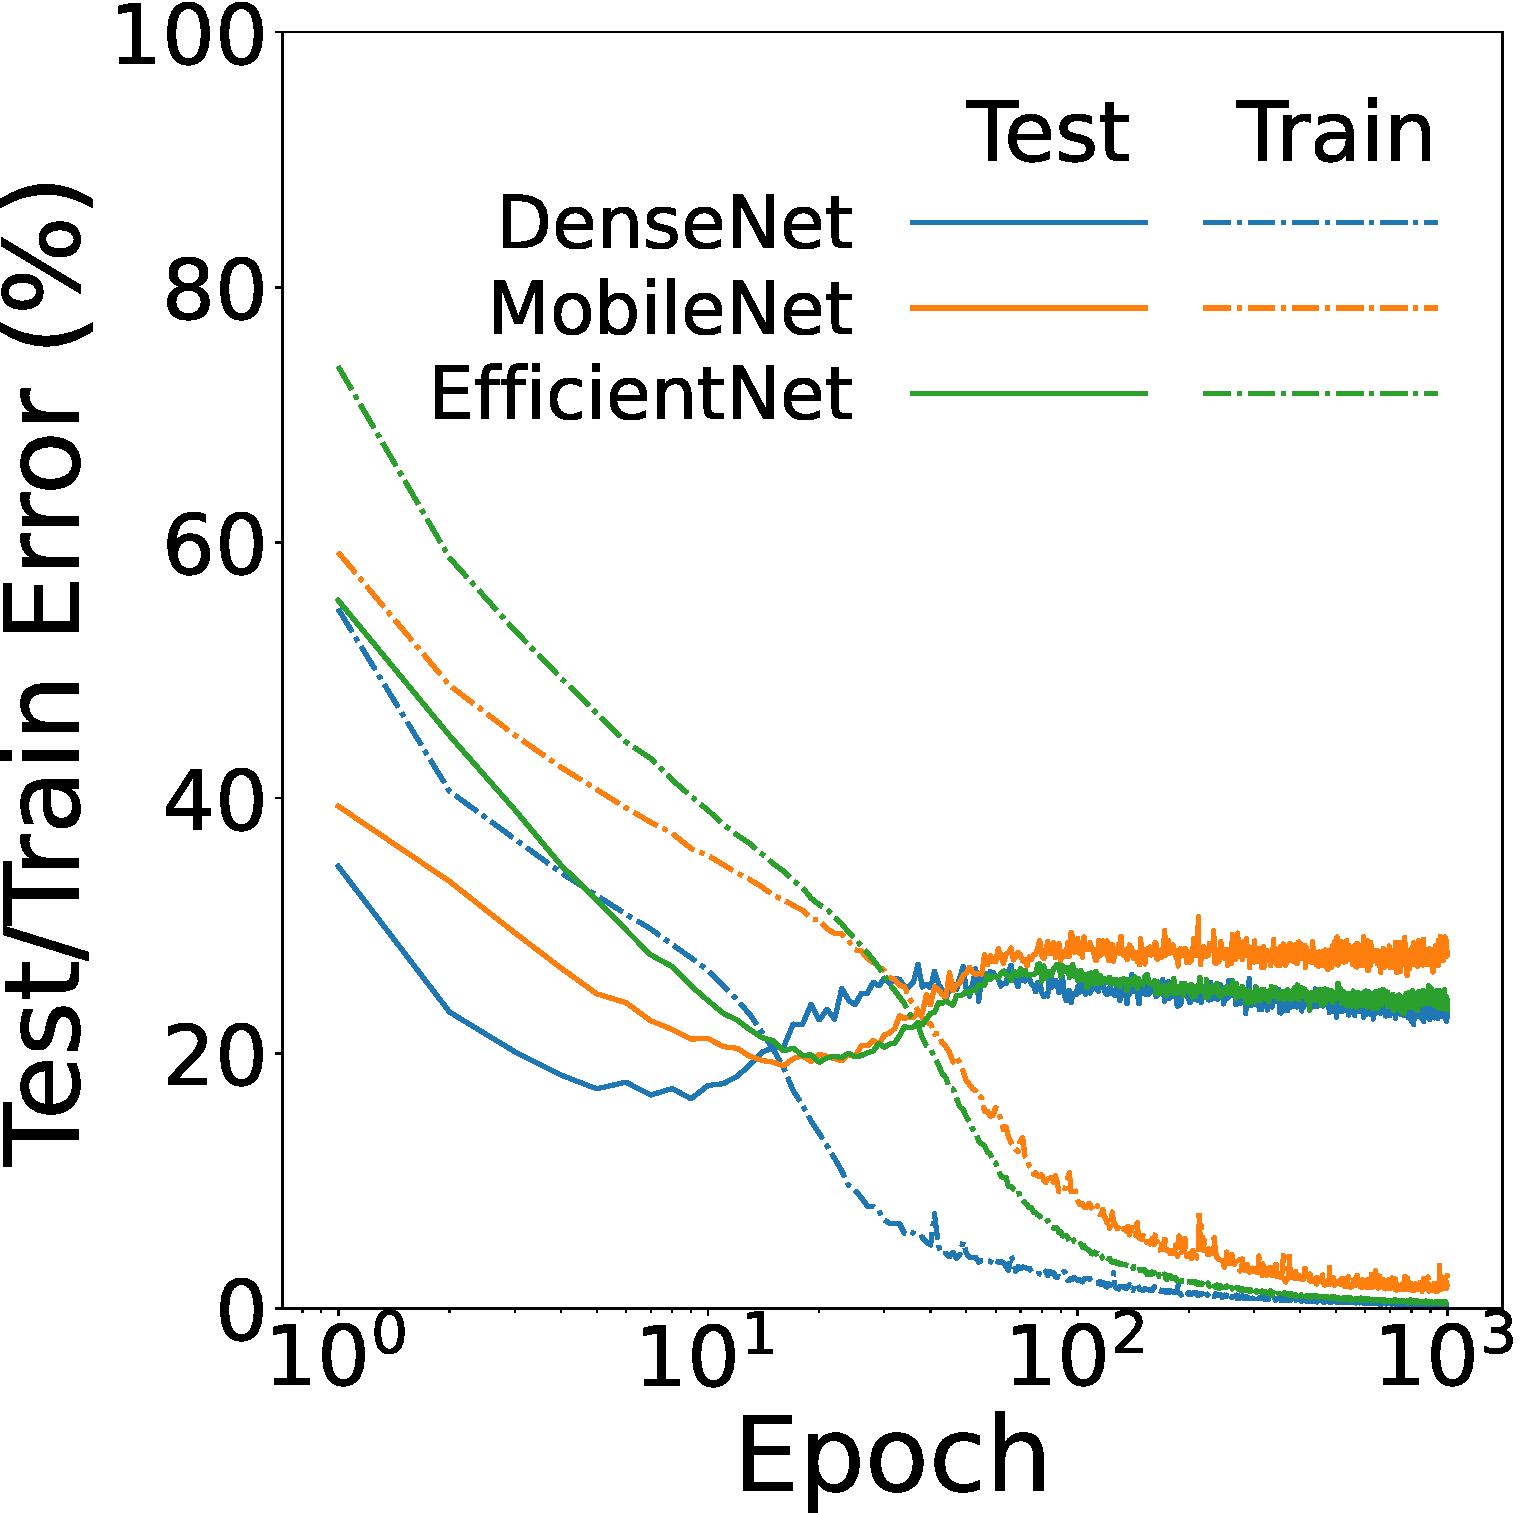
\includegraphics[keepaspectratio, width=0.45\linewidth]{fig/cnn_model_learning_curv.pdf} &
       \hspace{5pt} 
      %---- 2番目の図 --------------------------
      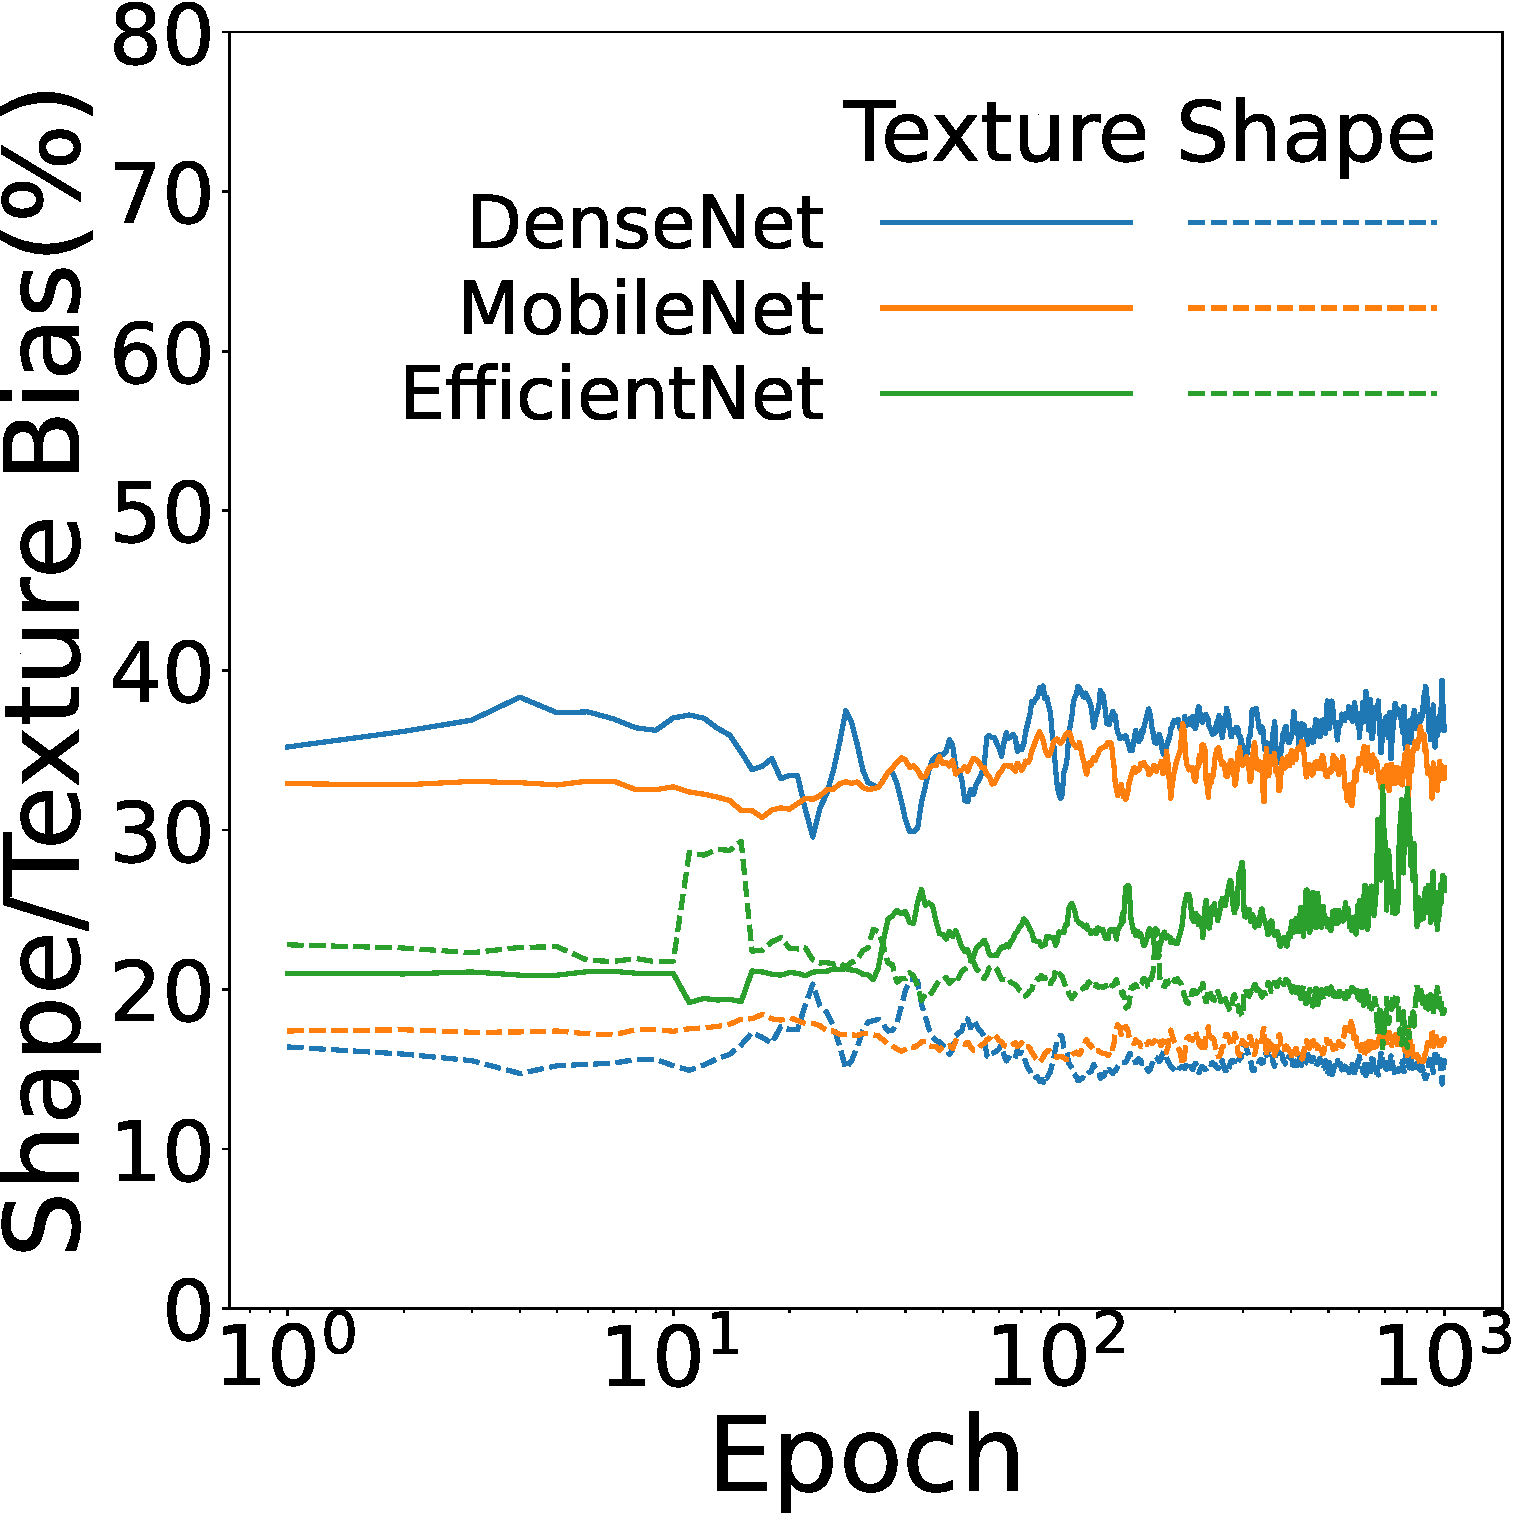
\includegraphics[keepaspectratio, width=0.45\linewidth]{fig/cnn_model_sha_tex.pdf}
   \end{tabular}
\caption[Learning process under various size conditions of CNN models.]{Learning process under various size conditions of CNN models. Left: train/test errors Right: shape/texture bias values.}
% Learning curve graphs for double descent and shape/texture bias for different models. \textbf{Left}:learning curve. \textbf{Right}:model's bias shift.}
\label{fig:comp_cnn_model}
\end{figure}

\begin{table}[htb]
    \centering
    \caption{
    % sample
    Correlation coefficients and scores in Phase 1, 2 and Phase 3 for different CNN models.
    }
    \scalebox{1.2}{
    \begin{tabular}{c|SSc|SSc} 
    \toprule[0.8pt]
    \multirow{2}{*}{CNN}  &  \multicolumn{3}{c|}{Correlation of Phase1,2} &  \multicolumn{3}{c}{Correlation of Phase3}\\
     \cline{2-7}
             & {SB} & {TB} & Score & {SB} & {TB} & Score \\
     \midrule[0.5pt]
    DenseNet &0.326&-0.322 & 0.324 & 0.293&-0.289 & 0.291\\
    MobileNet &-0.506&0.511 & 0.509&-0.016&0.036 & 0.026\\
    EfficientNet &-0.029&0.000 & 0.014&0.316&-0.343 & 0.330\\
    \toprule[0.8pt]
    \end{tabular}
    }
    \label{tab:corr_CNN_model}
\end{table}

\newpage

\subsection[Batch size]{Batch size (see \cref{fig:comp_batchsize} and \cref{tab:corr_batchsize})}
バッチサイズを変更した場合における,二重降下と形状・テクスチャ偏重度の推移への影響を検証した.異なるバッチサイズを使用した場合の結果を\cref{fig:comp_cnn_model}に,定量的な評価のための表を\cref{tab:corr_CNN_model}に示す.バッチサイズの減少に従って,テスト誤り率の曲線が右上にシフトしている.また,形状・テクスチャ偏重度の推移も,曲線の大きく落ち込んでいるところに注目すると,バッチサイズの減少に従って右にシフトしているよう見受けられる.定性的には,どの条件も相関を示していない.また,バッチサイズ4においては,定義した手法においては,Phaseを分割不可能であったため,データなしとしている.

このような二重降下の挙動の差異について,バッチサイズの低下によってepochあたりのイテレーション数は増加するため,バッチサイズが少ないほど,二重降下の挙動が右にシフトするのは予期しない結果となった.しかし,バッチサイズの増加によって学習の安定性が上昇するため,この影響であると考えられる.加えて,バッチサイズの増加につれて,右にシフトするのかについては,検証の余地がある.

\begin{figure}[htb]
\centering
   \begin{tabular}{cc}
      %---- 最初の図 ---------------------------
      \hspace{-5mm}
      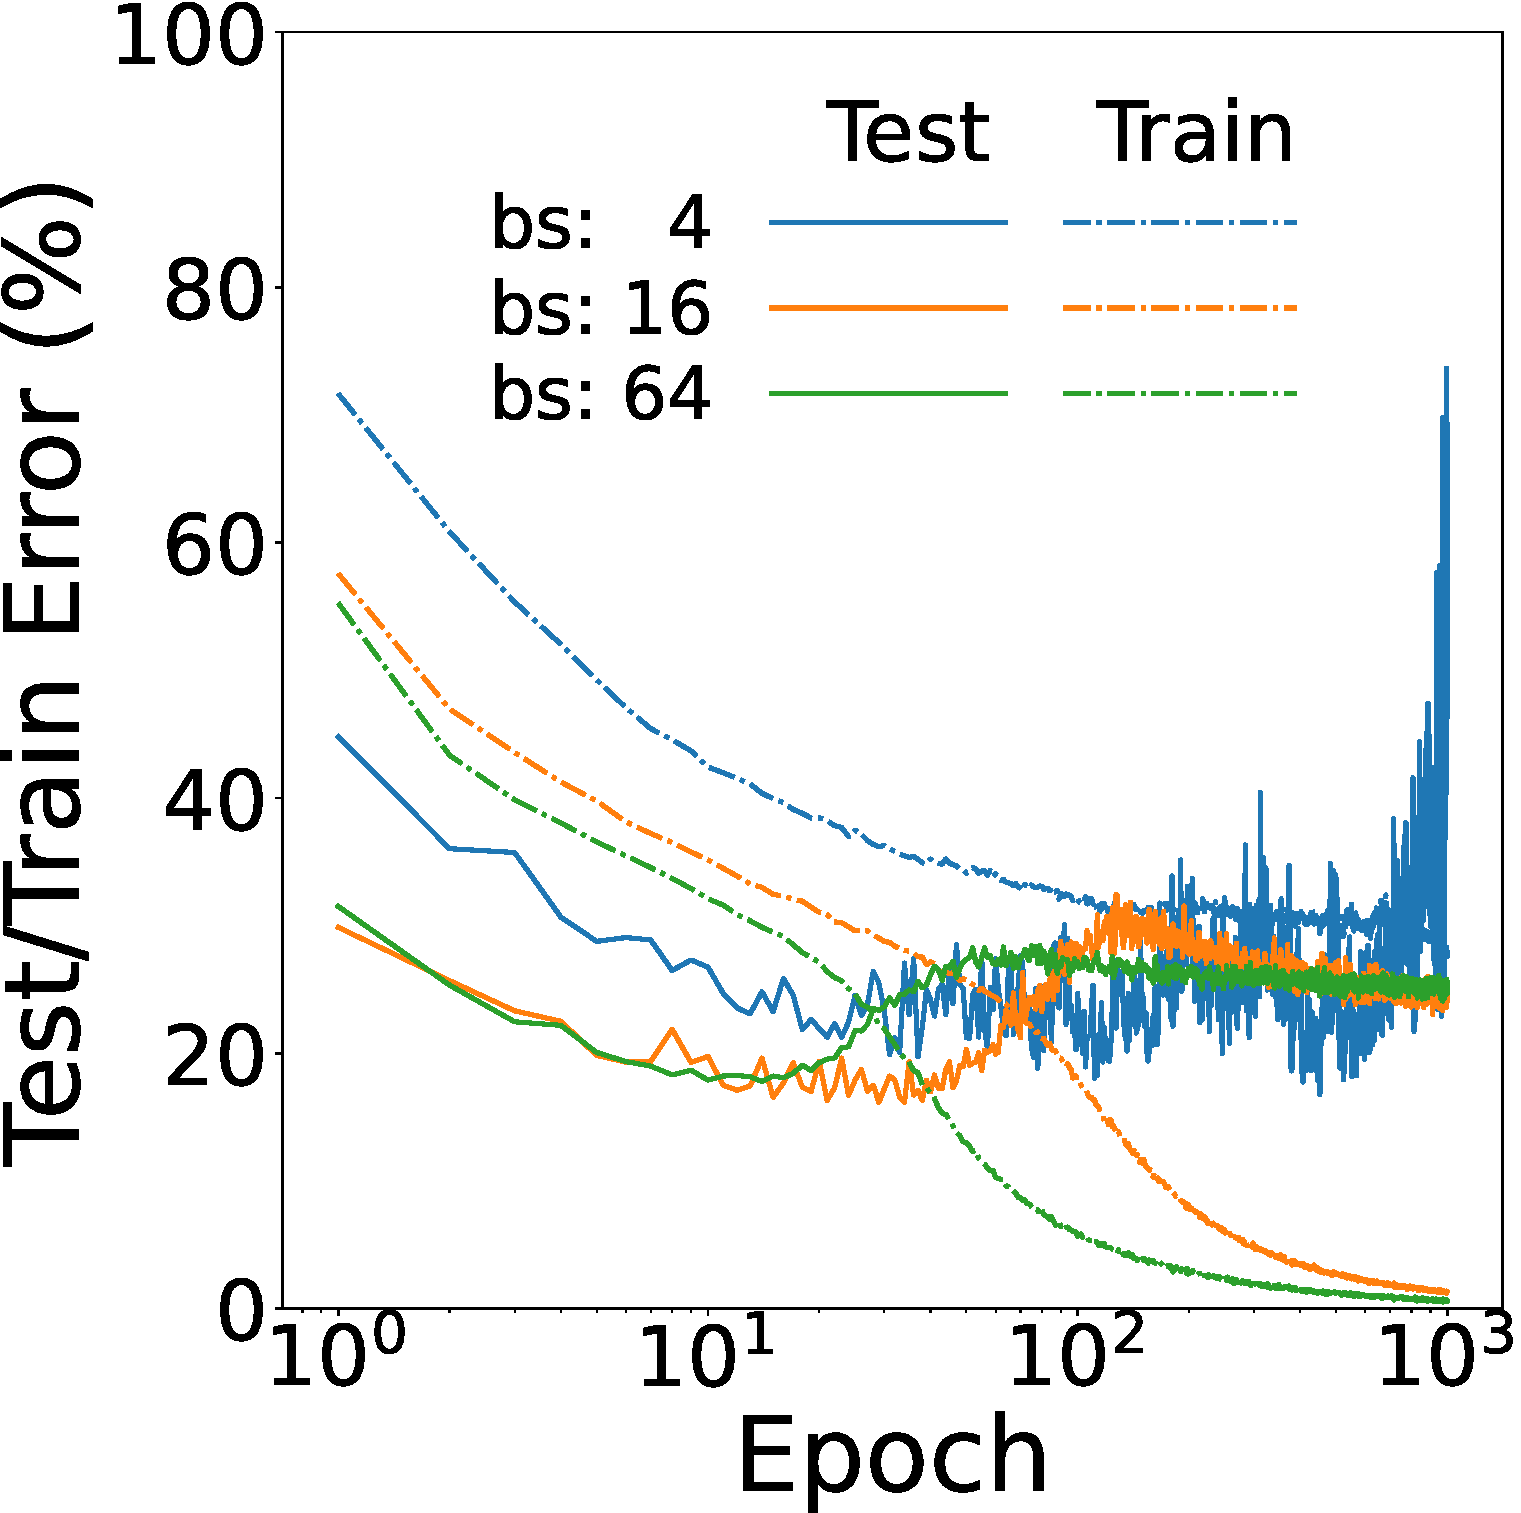
\includegraphics[keepaspectratio, width=0.45\linewidth]{fig/batchsize_learning_curv.pdf} &
        \hspace{5pt} 
      %---- 2番目の図 --------------------------
      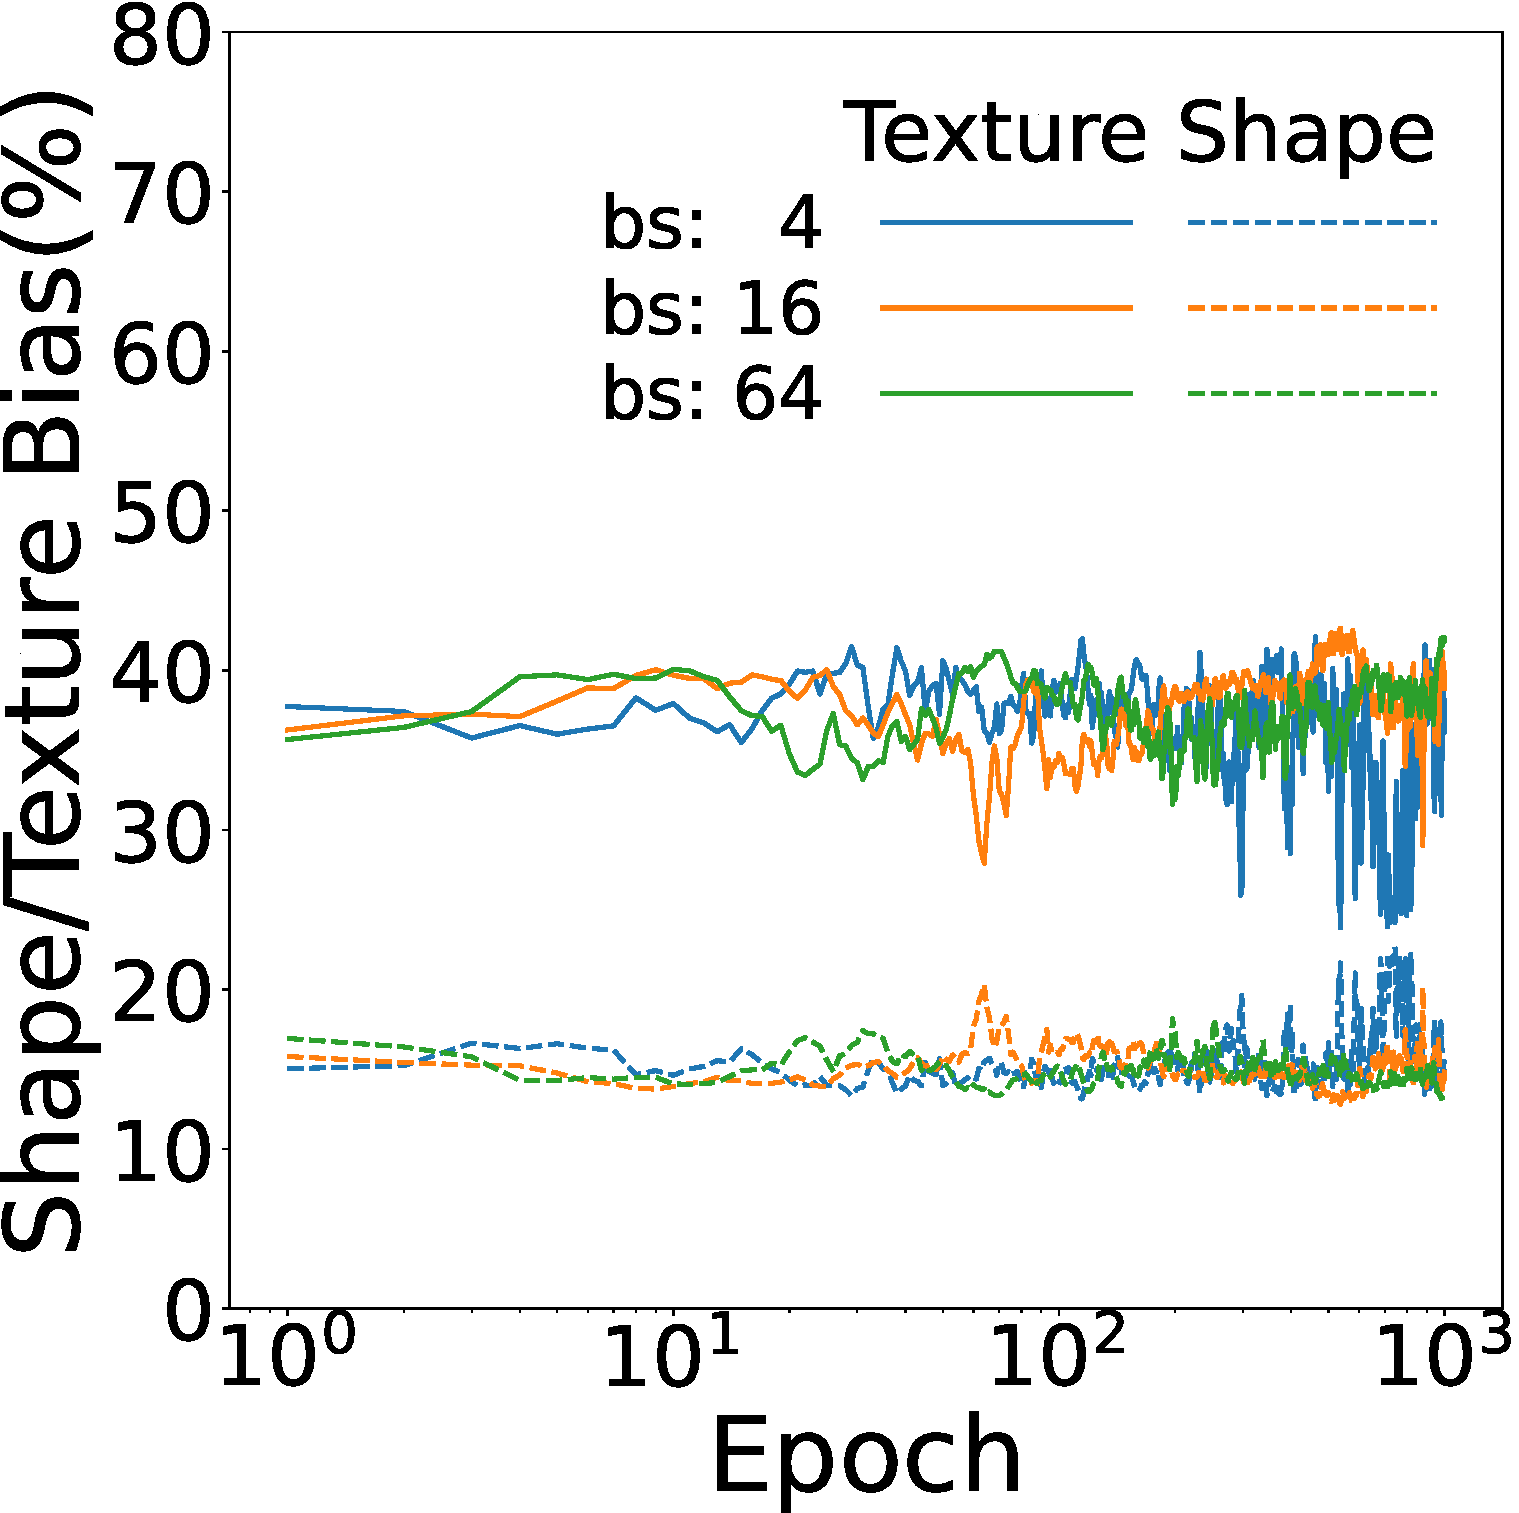
\includegraphics[keepaspectratio, width=0.45\linewidth]{fig/batchsize_sha_tex.pdf}
   \end{tabular}
\caption[Learning process under various batch size conditions.]{Learning process under various batch size conditions. Left: train/test errors Right: shape/texture bias values.}
%Learning curve graphs for double descent and shape/texture bias for different label noise. \textbf{Left}:learning curve. \textbf{Right}:model's bias shift.}
\label{fig:comp_batchsize}
\end{figure}

\begin{table}[htb]
    \centering
    \caption{
    % sample
    Correlation coefficients and scores in Phase 1, 2 and Phase 3 for different CNN models.
    }
    \scalebox{1.2}{
    \begin{tabular}{c|SSc|SSc} 
    \toprule[0.8pt]
    \multirow{2}{*}{batch size}  &  \multicolumn{3}{c|}{Correlation of Phase1,2} &  \multicolumn{3}{c}{Correlation of Phase3}\\
     \cline{2-7}
             & {SB} & {TB} & Score & {SB} & {TB} & Score \\
     \midrule[0.5pt]
    4 & N/A & N/A & N/A & N/A & N/A & N/A \\
    16 &0.249&-0.206 & 0.227 &-0.186&0.154 & 0.170\\
    64 &0.090&-0.065 & 0.077 &0.108&-0.101 & 0.105\\
    \toprule[0.8pt]
    \end{tabular}
    }
    \label{tab:corr_batchsize}
\end{table}

\newpage

\subsection[Label Noise]{Label Noise (see \cref{fig:comp_ln} and \cref{tab:corr_ln})}

ラベルノイズの増加は,二重降下の観測において重要なパラメータの一つである.そのため,特に偏重度の推移に対して,どのような影響を与えるか,ラベルノイズの割合を変更し検証を行った.ラベルノイズの増加による,二重降下と形状・テクスチャ偏重度の推移への影響を検証した結果を\cref{fig:comp_ln}に示す.ラベルノイズの割合は,20\%に加えて,40\%,60\%と変化させた条件で行った.相関係数の定量評価を\cref{tab:corr_ln}に示す.テスト誤り率の推移からわかるように,ラベルノイズが大きくなるにつれて二重降下のPhase2における変動幅が大きくなっている.しかし,形状とテクスチャ偏重度を見ると,ラベルノイズの割合に関係なく,形状・テクスチャ偏重度の明確な傾向が観察される.特に,テクスチャ偏重度では,ラベルノイズが大きくなるにつれて,上昇から下降へのシフトのタイミングが遅れているように見える.各条件の相関を比較すると,40\%の場合には相関は見られていないが,60\%の場合はScoreが0.579と,相関がみられている.このことから,ラベルノイズが大きくなるにつれて,偏重度の推移が遅くなる可能性がある.

\begin{figure}[htb]
\centering
   \begin{tabular}{cc}
      %---- 最初の図 ---------------------------
      \hspace{-5mm}
      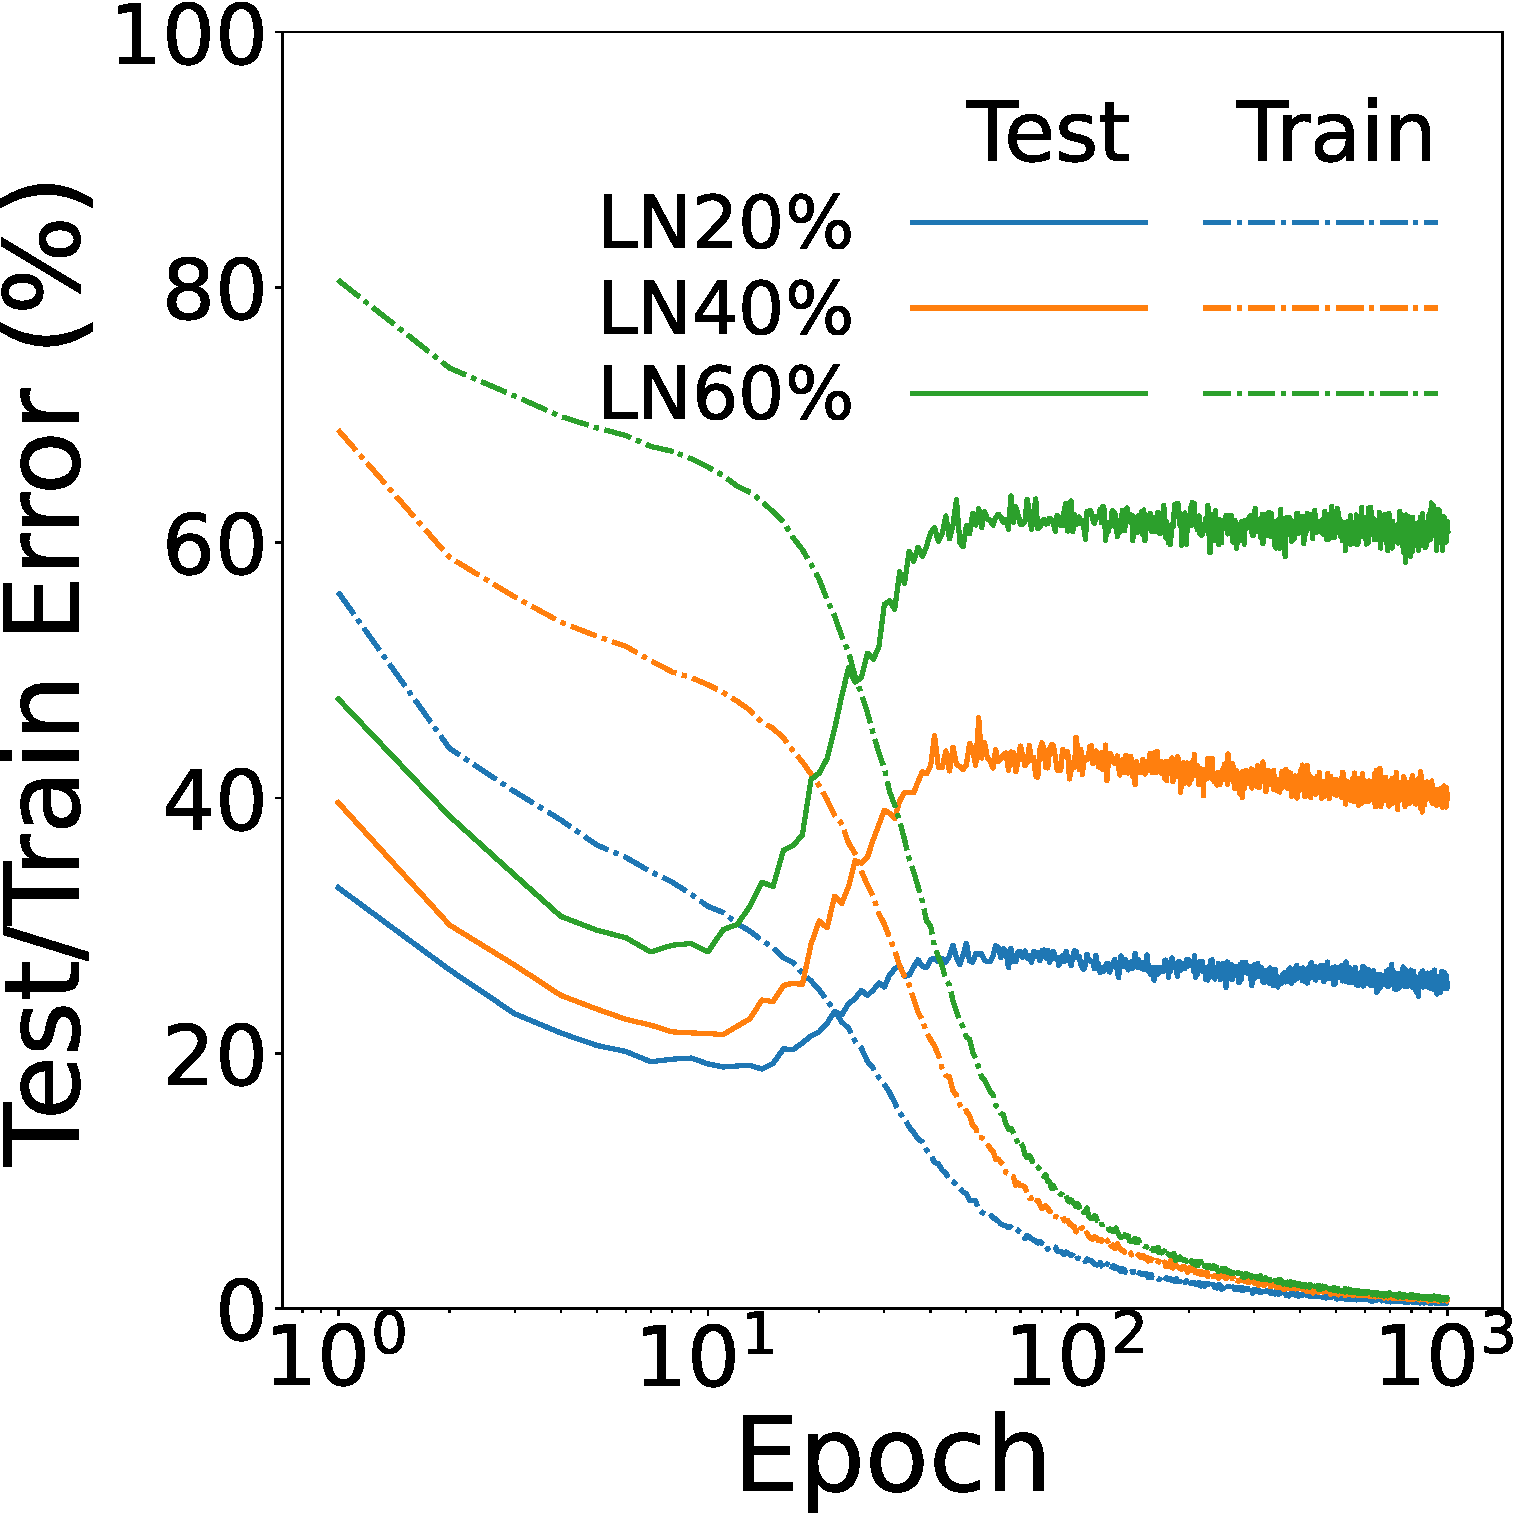
\includegraphics[keepaspectratio, width=0.45\linewidth]{fig/ln_learning_curv.pdf} &
       \hspace{5pt} 
      %---- 2番目の図 --------------------------
      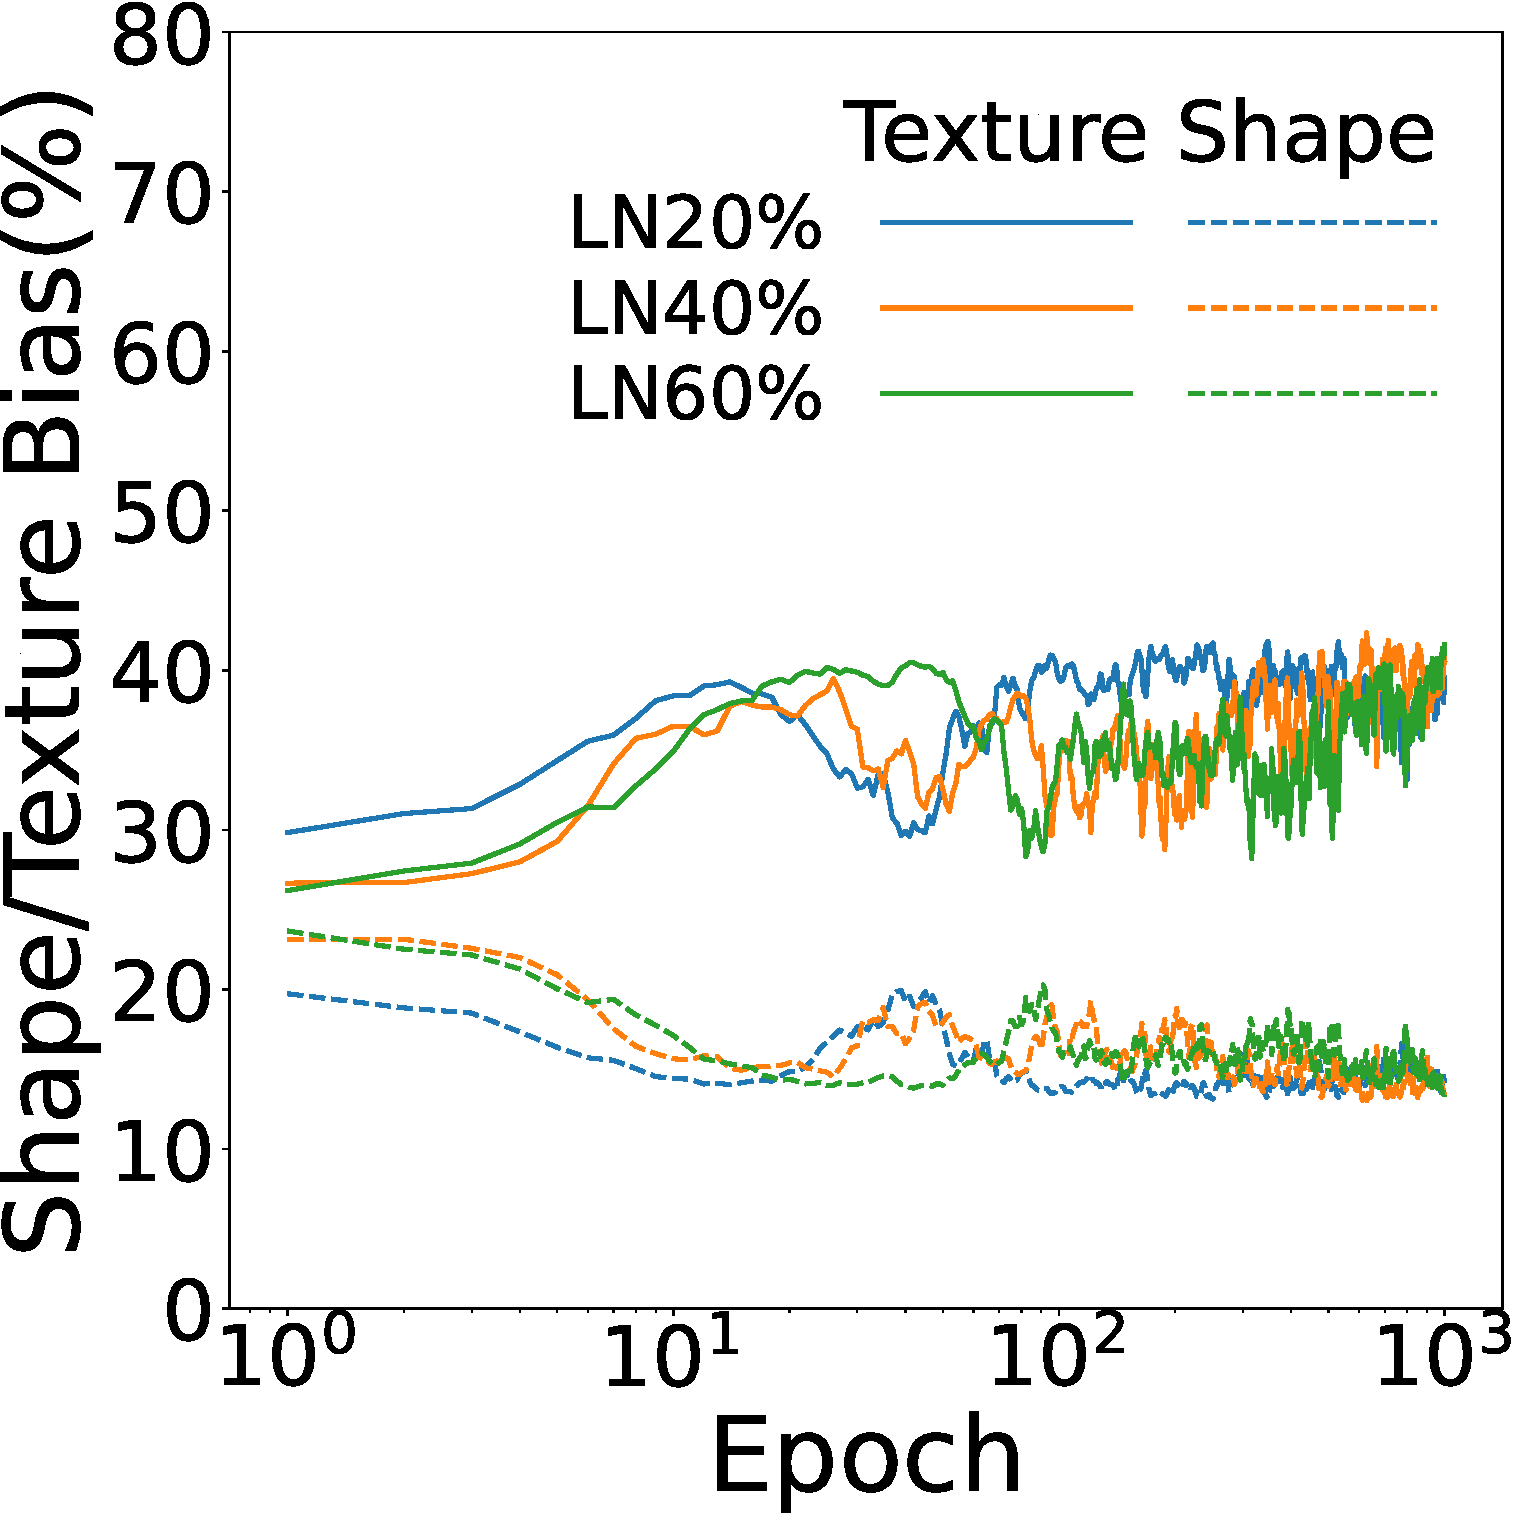
\includegraphics[keepaspectratio, width=0.45\linewidth]{fig/ln_sha_tex.pdf}
   \end{tabular}
\caption[Learning process under various label noise conditions.]{Learning process under various label noise conditions. Left: train/test errors Right: shape/texture bias values.}
%Learning curve graphs for double descent and shape/texture bias for different label noise. \textbf{Left}:learning curve. \textbf{Right}:model's bias shift.}
\label{fig:comp_ln}
\end{figure}

\begin{table}[htb]
    \centering
    \caption[Correlation coefficients and scores in Phase 1, 2 and Phase 3 on different label noise.]{
    % 異なるラベルノイズに対するPhase1,Phase2,Phase3の相関係数とスコア.テスト誤差と形状・テクスチャの偏りの相関係数(SB, TB)と,これら2つの相関係数から計算されたスコアを示す.
    Correlation coefficients and scores in Phase 1, 2 and Phase 3 on different label noise. It shows the correlation coefficients (SB, TB) between test error and shape/texture bias and the score calculated from these two correlation coefficients.
    }
    % \begin{tabular}{c|c|c} 
    % \toprule[0.8pt]
    % Label noise  & Correlation area &  score\\
    %  \midrule[0.5pt]
    % 20\%  & Stage1,2 (2-41) &0.778\\
    % 40\% & Stage1,2 (2-114) &0.048\\
    % 60\% & Stage1,2 (2-36) &0.579\\
    % \toprule[0.8pt]
    % \end{tabular}
    \scalebox{1.2}{
    \begin{tabular}{c|SSc|SSc} 
    \toprule[0.8pt]
    \multirow{2}{*}{Label Noise}  &  \multicolumn{3}{c|}{Correlation of Phase1,2} &  \multicolumn{3}{c}{Correlation of Phase3}\\
     \cline{2-7}
             & {SB} & {TB} & Score & {SB} & {TB} & Score \\
     \midrule[0.5pt]
    20\% &0.778&-0.778 & 0.778 & -0.026&0.118 & 0.072\\
    40\% & 0.004 & -0.091 & 0.048 &0.451&-0.487 & 0.469\\
    60\% &-0.560 & 0.598 & 0.579 & 0.122 & -0.142 & 0.132\\
    \toprule[0.8pt]
    \end{tabular}
    }
    \label{tab:corr_ln}
\end{table}

\newpage

\subsection[Seed]{Seed (see \cref{fig:comp_seed} and \cref{tab:corr_seed})}
機械学習の実験においては,再現性を担保するために,シード値を固定して,実験を行う場合がある.そのため,シード値を変更した場合における二重降下と形状・テクスチャ偏重度の推移への影響を検証した.使用したシード値は,元の条件である42に加えて0,1を使用した.0,1,42は機械学習の分野においてもっともよく使用されるシード値である.シード値を変更した場合の結果を\cref{fig:comp_seed}に,定量的な評価のための表を\cref{tab:corr_seed}に示す.シード値が42の場合において,ベースラインの結果と異なっているが,異なる計算機環境で実験で行った結果であることに留意されたい.
すべての場合において,二重降下がほとんど一致している.一方で,例えばテクスチャ偏重度は,すべての条件において,上昇して下降する傾向が見られる.しかし,定量的には,すべての条件において二重降下と形状・テクスチャ偏重度との相関は捉えられなかった.

事前学習したパラメータを使用する場合,事前学習をしたパラメータを読み込んだのちに,モデルが持つ全結合層のみ再度の初期化を行うことが一般的である.この実験では,シード値を変更しているが,畳み込み層は事前学習したパラメータを使用しているため,モデルが持つ全結合層のパラメータのみに差異があると考えられる.そのため,全結合層におけるパラメータの初期値が,二重降下にはさほど影響を与えないが,偏重度の推移には大きく影響を与えていると推察される.

\begin{figure}[htb]
\centering
   \begin{tabular}{cc}
      %---- 最初の図 ---------------------------
      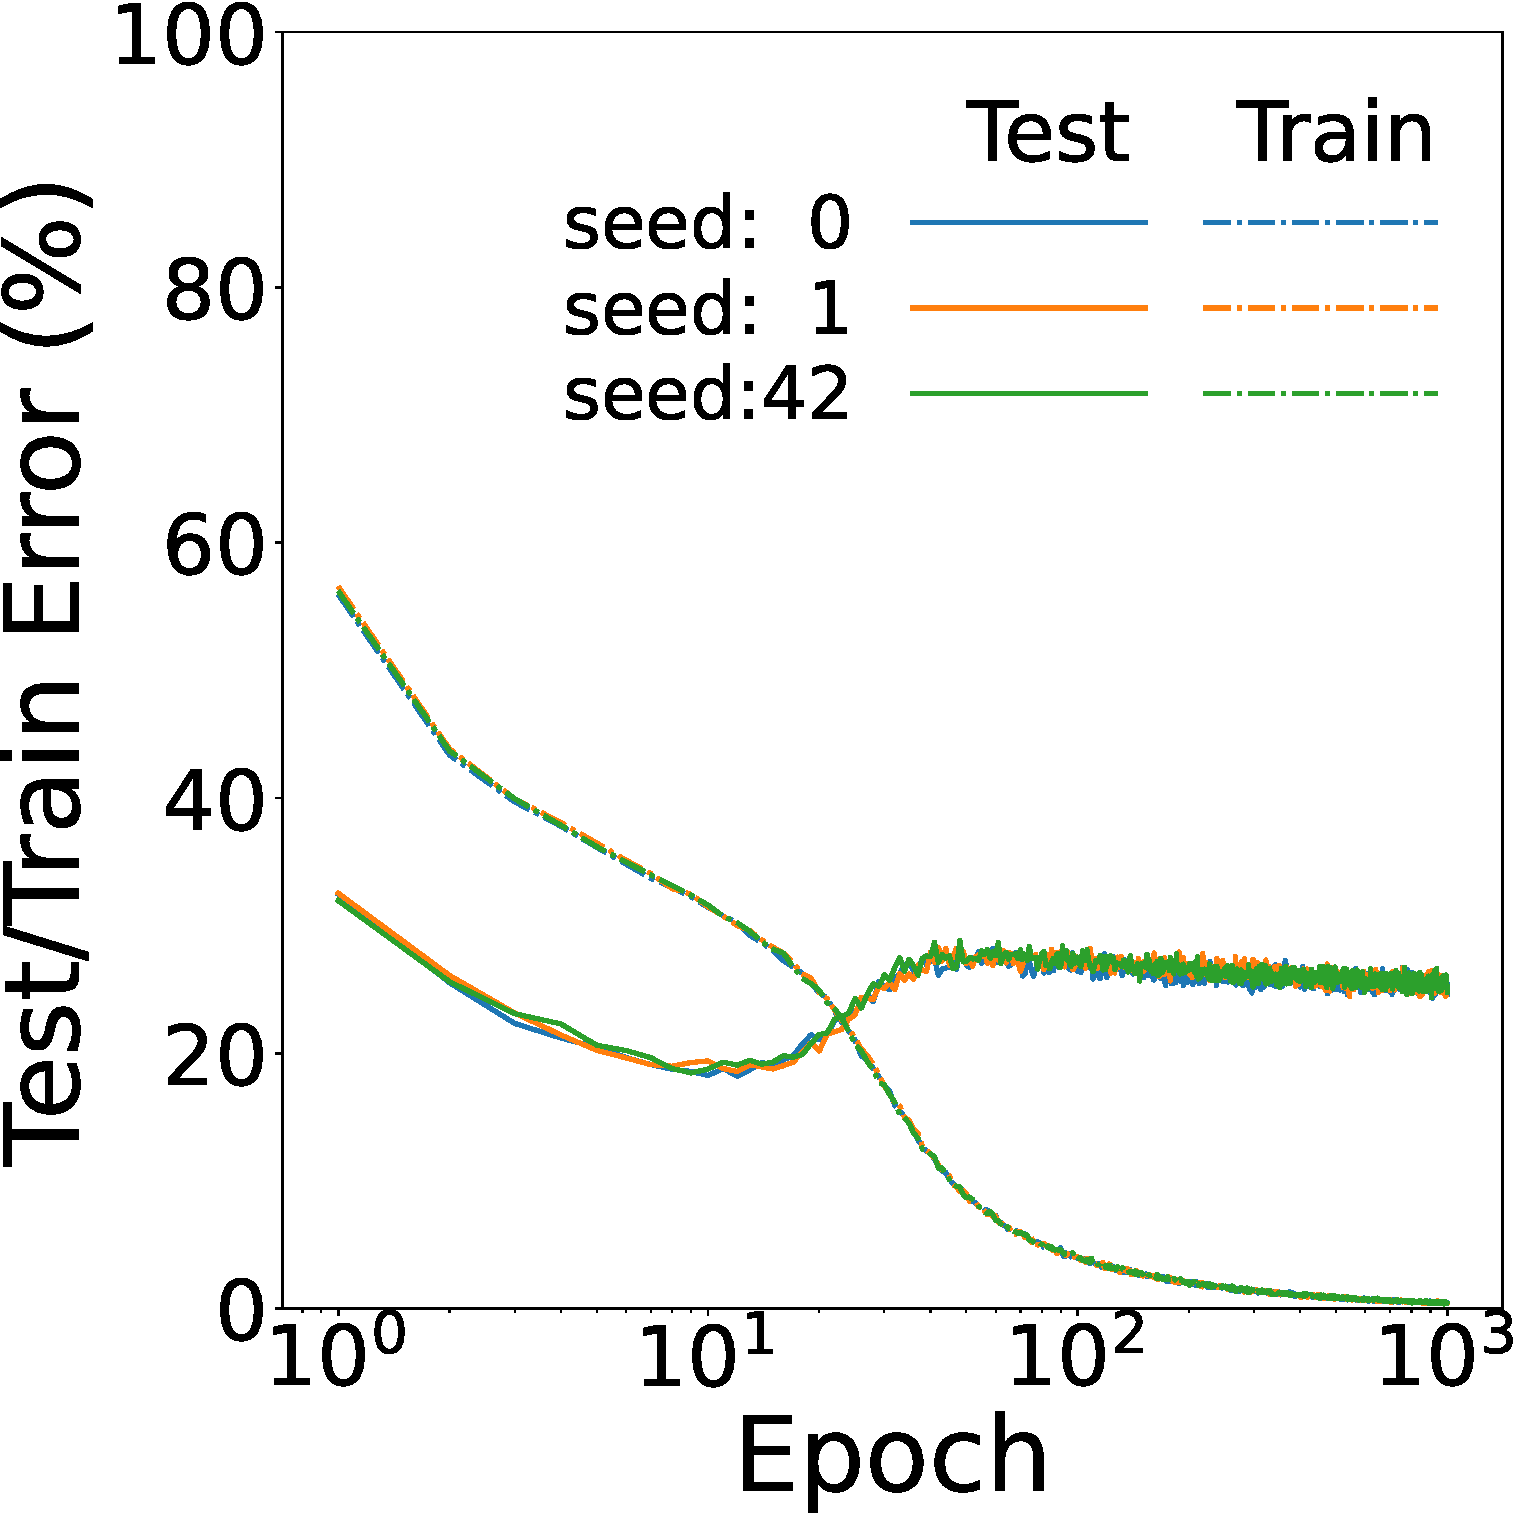
\includegraphics[keepaspectratio, width=0.45\linewidth]{fig/seed_learning_curv.pdf} &
       \hspace{5pt} 
      %---- 2番目の図 --------------------------
      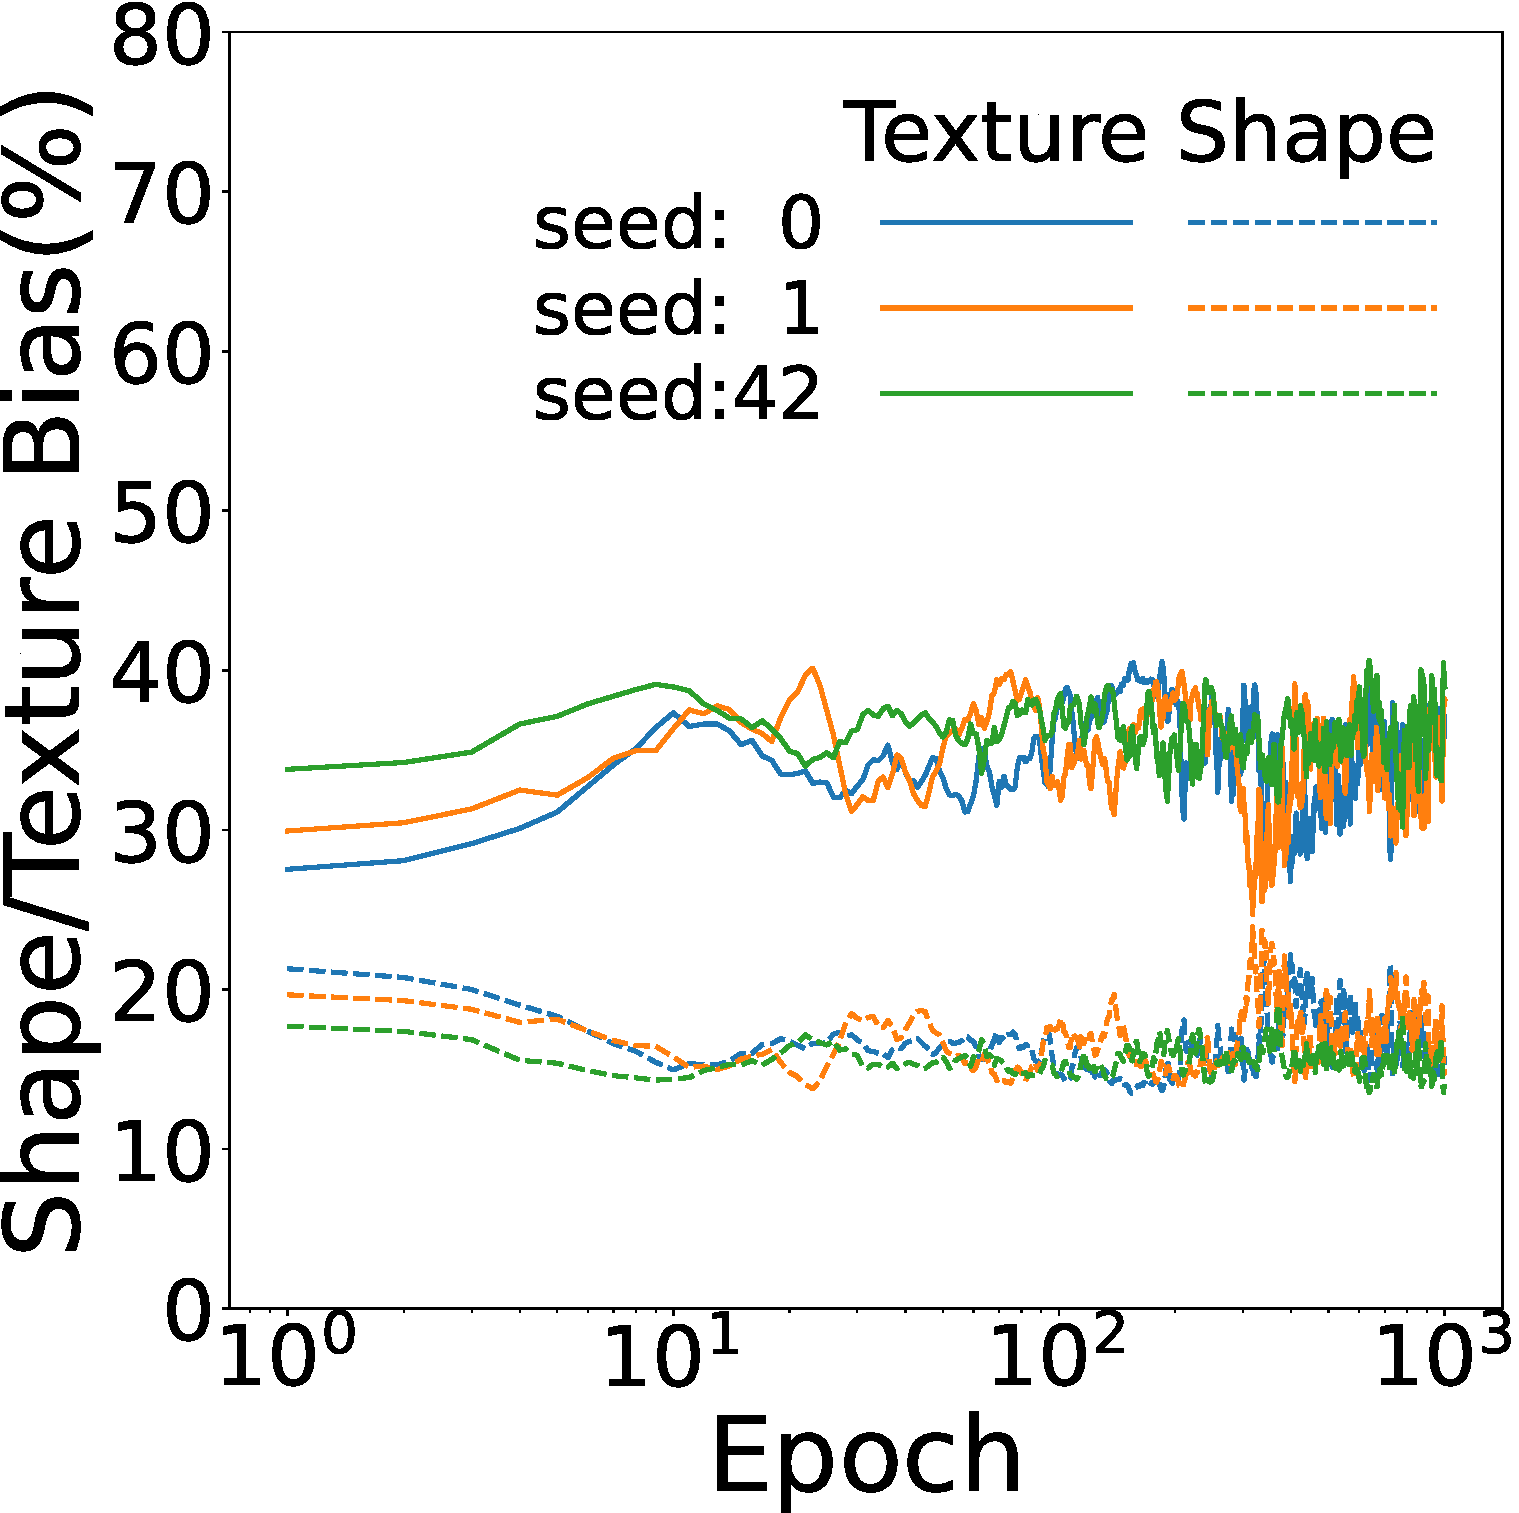
\includegraphics[keepaspectratio, width=0.45\linewidth]{fig/seed_sha_tex.pdf}
   \end{tabular}
\caption[Learning process under various seed conditions.]{Learning process under various seed conditions. Left: train/test errors Right: shape/texture bias values.}
%Learning curve graphs for double descent and shape/texture bias for different label noise. \textbf{Left}:learning curve. \textbf{Right}:model's bias shift.}
\label{fig:comp_seed}
\end{figure}

\newpage

\begin{table}[htb]
    \centering
    \caption[Correlation coefficients and scores in Phase 1, 2 and Phase 3 under various seed conditions.]{
    % 異なるラベルノイズに対するPhase1,Phase2,Phase3の相関係数とスコア.テスト誤差と形状・テクスチャの偏りの相関係数(SB, TB)と,これら2つの相関係数から計算されたスコアを示す.
    Correlation coefficients and scores in Phase 1, 2 and Phase 3 on different label noise. It shows the correlation coefficients (SB, TB) between test error and shape/texture bias and the score calculated from these two correlation coefficients.
    }
    % \begin{tabular}{c|c|c} 
    % \toprule[0.8pt]
    % Label noise  & Correlation area &  score\\
    %  \midrule[0.5pt]
    % 20\%  & Stage1,2 (2-41) &0.778\\
    % 40\% & Stage1,2 (2-114) &0.048\\
    % 60\% & Stage1,2 (2-36) &0.579\\
    % \toprule[0.8pt]
    % \end{tabular}
    \scalebox{1.2}{
    \begin{tabular}{c|SSc|SSc} 
    \toprule[0.8pt]
    \multirow{2}{*}{Seed}  &  \multicolumn{3}{c|}{Correlation of Phase1,2} &  \multicolumn{3}{c}{Correlation of Phase3}\\
     \cline{2-7}
             & {SB} & {TB} & Score & {SB} & {TB} & Score \\
     \midrule[0.5pt]
    0 &0.034&-0.178 & 0.105 & -0.132& 0.133 & 0.132\\
    1 & 0.040 & -0.013 & 0.026 &-0.123&0.087 & 0.105\\
    42 &-0.015 & -0.087 & 0.051 & 0.069 & 0.017 & 0.043\\
    \toprule[0.8pt]
    \end{tabular}
    }
    \label{tab:corr_seed}
\end{table}

\newpage